\documentclass[]{report}
\usepackage{amsmath}
\usepackage{bm}
\usepackage{listings}
% % \textwidth 16cm \textheight 23.5cm
% \renewcommand{\baselinestretch}{1.2}
\usepackage{graphicx}
\usepackage{graphics}
\usepackage{epsfig}
\usepackage{color}
\usepackage{multirow}
\usepackage[colorlinks]{hyperref}
\usepackage{fancyhdr}
\usepackage{calc}
\usepackage[numbers]{natbib}
\usepackage{bibentry}
% underline tool
\usepackage[normalem]{ulem}
\usepackage{xcolor}
%\uline{foo}	Underlines foo
%\uuline{foo}	Double underlines foo
%\uwave{foo}	Underlines foo with a wavy line
%\sout{foo}	Strikesout foo
%\xout{foo}	Crosses out foo with ¡®/6¤7¡¯
% triple lines in colors
\makeatletter
\newcommand\uuuline{\bgroup\markoverwith%
   {%
     \textcolor{red}{\rule[-0.5ex]{2pt}{0.4pt}}%
     \llap{\textcolor{blue}{\rule[-0.7ex]{2pt}{0.4pt}}}%
     \llap{\textcolor{green}{\rule[-0.9ex]{2pt}{0.4pt}}}%
   }%
   \ULon}
\makeatother


\usepackage{amsmath,soul} % underline with a number
% usage example: $\underset{4}{\text{\ul{This is short text}}}$
% another package to use, but did not work for me.
% From: http://tex.stackexchange.com/questions/45341/labeling-underlined-text-over-multiple-lines
%\usepackage{soulpos}
%\ulposdef{\ulnumaux}{%
%   $\underset{\saveulnum}{\rule[-.7ex]{\ulwidth}{.4pt}}$}
%
%\newcommand{\ulnum}[2]{%
%  \def\saveulnum{#1}%
%  \ulnumaux{#2}}

% todo list and commands
\usepackage{todonotes}
%% to avoid the conflict with amths package % not working
%\makeatletter
%\providecommand\@dotsep{5}
%\makeatother
%\listoftodos\relax
\usepackage{makeidx}
\allowdisplaybreaks
% for eps transfering to pdf.
\usepackage[update,prepend]{epstopdf}
\usepackage{ifpdf}

\ifpdf
   \usepackage{graphicx}
   \usepackage{epstopdf}
   \epstopdfsetup{suffix=}
   \DeclareGraphicsRule{.eps}{pdf}{.pdf}{`epstopdf #1}
   \pdfcompresslevel=9
\else
   \usepackage{graphicx}
\fi
% subfig
\usepackage{mwe}
\usepackage{subfig}
% to fix a figure's position using [H] option of thec figure.
\usepackage{float}
% to use \lesssim and other math symbols
\usepackage{amssymb}


% self-defined short-cuts and commands

% packages we need for judging the operating system
% compile your tex file with option -shell-escape is required: 
% e.g. xelatex -shell-escape file.tex
\usepackage{pdftexcmds}
\usepackage{catchfile}
\usepackage{ifluatex}
\usepackage{ifplatform}

% judge platform and include correct definiation package
\ifwindows
	%\input{F:/Research/Works/Templates/Mydef.tex} % %
	\input{F:/Research/Works/Templates/Mydef.tex} % 
\else
	\input{/media/F/Research/Works/Templates/Mydef.tex} %
\fi

%\includeonly{VectorTensor}
% for table captions.
\usepackage{tabularx,ragged2e,booktabs,caption}





% % % % % % % % % % % % % % % % % % %

% Title Page
\title{Scattering problem in the Nanofiber Trapped Atom system}
\author{Xiaodong Qi and Ben Quinn Baragiola}

\makeindex

\begin{document}
\maketitle

\begin{abstract}
This is a study on the Nanofiber Trapped Atoms project (NaTA) in the perspective of scattering. 
\end{abstract}












\chapter{One atom trapped aside a nanofiber}

\section{Green function for the classical light}
In this section, we look at the case that only one atom is trapped aside the nanofiber. To be specific, we consider the following scenario: a laser beam propagates through a nanofiber along $ z $ direction; a Cesium (Cs) atom (can be other atoms) allocates at $ \mathbf{r}_{atom} =\mathbf{r}'$ close by the nanofiber, and responds to the optical field. Due to the response of the atom, a light is re-emitted
from the atom with a phase shift propagating in all directions, and interferes with the guided mode, which causes attenuation and a change of the index of refraction\index{index of refraction} of the nanofiber effectively. 

We assume that the nanofiber is a infinite long cylinder with a radium of $ a $ (in our cases, $ a<\lambda $, where $ \lambda $ is the wavelength of the laser beam). The laser beam propagating in the nanofiber generates an electrical field given by
\begin{equation}
\mathbf{E}_0(\br,t)=\boldsymbol{\mathcal{E}}_0(\br)e^{-i\omega t} %+\frac{1}{2}\mathrm{c.c.}
=\mathcal{E}_0(\br)\mathbf{u}_0(\br)e^{-i\omega t}, %+\frac{1}{2}\mathrm{c.c.},
\label{Ert0}
\end{equation}
where $\omega$ is the angular frequency and $\boldsymbol{\mathcal{E}}_0(\br)=\mathcal{E}_0\mathbf{u}_0$ is the positive-frequency electric field envelope,
with $\mathcal{E}_0(\br)$ and $\mathbf{u}_0(\br)$ being the field amplitude and the polarization vector at $ \br $, respectively.
In general, $\mathcal{E}(\br)$ is a complex scalar and $\mathbf{u}(\br)$ is a complex unit vector. 

We assume the nanofiber is a linear medium with no absorption to the traveling wave. The refractive intrinsic index\index{refractive index} of the nanofiber can be given by
\begin{align}
n_0(\br) = \begin{cases} 
n_1=1.46, &\quad r_\perp \leq a,\\
n_2=1, &\quad r_\perp >a,
\end{cases} 
\end{align}
where we have set the $ z $-axis to be the symmetric center of the nanofiber and $ r_\perp =\sqrt{x^2+y^2} $. We would like to determine the form of the scattered field $ \boldsymbol{\mathcal{E}}_s(\br) $, and the total field $ \boldsymbol{\mathcal{E}}(\br)=\boldsymbol{\mathcal{E}}_0(\br)+\boldsymbol{\mathcal{E}}_s(\br) $. Formally, the total time-dependent electrical field can be rewritten as 
\begin{equation}
\mathbf{E}(\br,t)=\boldsymbol{\mathcal{E}}(\br)e^{-i\omega t} %+\frac{1}{2} \mathrm{c.c.}
=\mathcal{E}(\br)\mathbf{u}(\br)e^{-i\omega t}, %+\frac{1}{2}\mathrm{c.c.},
\label{Ert}
\end{equation}

The total field will satisfy the \textit{Maxwell-Helmholtz equation}\index{Maxwell-Helmholtz equation} that
\begin{align}
\left[ \nabla\times\nabla\times-\frac{\omega^2}{c^2}n^2(\br) \right] \boldsymbol{\mathcal{E}}(\br) &=0. \label{MaxwellHelmholtz0}
\end{align}
Notice that the total index of refraction $ n(\br) $ we used above has already included the scattering effect caused by the atom on the nanofiber, which usually has a complicated form. It is not in general possible to solve the differential equation as given above. The solution to the Maxwell-Helmholtz equation\index{Maxwell-Helmholtz equation} with $ n(\br)=1 $, however, are much more tractable, so we subtract $ \frac{\omega^2}{c^2} \boldsymbol{\mathcal{E}}(\br)$ to each side of Equ.~\ref{MaxwellHelmholtz0} and add $ \frac{\omega^2}{c^2}n(\br) \boldsymbol{\mathcal{E}}(\br) $ to give
\begin{align}
\left[ \nabla\times\nabla\times - \frac{\omega^2}{c^2} \right] \boldsymbol{\mathcal{E}}(\br) &= \frac{\omega^2}{c^2} \boldsymbol{\chi}(\br) \boldsymbol{\mathcal{E}}(\br),
\end{align}
where we have defined the electric susceptibility\index{electric susceptibility} $ \boldsymbol{\chi}(\br)=n^2(\br)-1=\varepsilon_r(\br)-1 = \delta(\br-\mathbf{r}')\boldsymbol{\alpha} \, (r_\perp>a)$ where $ \varepsilon_r(\br) $ is the relative permittivity\index{permittivity!relative permittivity} or dielectric constant\index{dielectric constant} at $ \br $ and $ \boldsymbol{\alpha} $ is the polarizability\index{polarizability} of the atom~\footnote{\textcolor{red}{This electric susceptibility needs to be fixed.} Aside on multiple atoms case: if there are many atoms distributed along the nanofiber, we can in general use 
$\boldsymbol{\chi}(\br)=\sum_i \delta(\br-\br_{i})\boldsymbol{\alpha}^i$,
where $ i $ counts over all atoms.}. This equation above has a source term 
\begin{align}
S(\br)=\frac{\omega^2}{c^2} \boldsymbol{\chi}(\br),% \boldsymbol{\mathcal{E}}(\br),
\end{align}
and can be solved by solving the corresponding Green function\index{Green function} in the frequency domain
\begin{align}
\left[ \nabla\times\nabla\times - \frac{\omega^2}{c^2} \right] \mathbf{G}(\br,\br') &= \mathbf{I}\delta(\br-\br').
\end{align}
The solution for the Green function\index{Green function} in free space is 
\begin{align}
\mathbf{G}(\br,\br') =\frac{e^{i\mathbf{k}\cdot (\mathbf{r}-\br')}}{|\br-\br'|}.
\end{align}

\textcolor{red}{Assuming the boundary contributions vanish}, we may have
\begin{align}
\boldsymbol{\mathcal{E}}(\br) &= \boldsymbol{\mathcal{E}}_0 (\br) + \int_V S(\br') \boldsymbol{\mathcal{E}}(\br') \frac{e^{i\mathbf{k}\cdot \mathbf{R}}}{R} \mathrm{d}^3 r', \label{Etotal0}
\end{align}
where $ \boldsymbol{\mathcal{E}}_0 (\br) $ is the homogeneous Maxwell-Helmholtz equation\index{Maxwell-Helmholtz equation!homogeneous Maxwell-Helmholtz equation} in the limit that $ S(\br)\longrightarrow 0 $, $ \mathbf{R}=\br-\mathbf{r}' $. Therefore, the scattering field is
\begin{align}
\boldsymbol{\mathcal{E}}_s(\br) &=  \int_V S(\br') \boldsymbol{\mathcal{E}}(\br') \frac{e^{i\mathbf{k}\cdot \mathbf{R}}}{R} \mathrm{d}^3 r'\\
&= \int_V \frac{\omega^2}{c^2} \boldsymbol{\chi}(\br') \boldsymbol{\mathcal{E}}(\br') \frac{e^{i\mathbf{k}\cdot \mathbf{R}}}{R} \mathrm{d}^3 r'.
\end{align}



In general, scattering problems cannot be solved analytically, due to the presence of the complicated scattered field. By the use of Green function method, we have converted our differential equation for the scattered field into volume integral equations. They are very important since they form the basis for various formalisms such as the \textit{method of moments}\index{method of moments}, the \textit{Lippmann-Schwinger equation}\index{Lippmann-Schwinger equation}, and the \textit{coupled dipole method}\index{coupled dipole method}. In general, these integral equations can be solved numerically using the methods mentioned above. Alternatively, we may develop a Liouville–Neumann series\index{Liouville–Neumann series} solution to the equation, namely the Born series\index{Born series}.

The Born series is typically derived by assuming that the scattering potential is very
weak, and may be written as $ S(\br)\rightarrow \delta S(\br) $, where $ \delta $ is a dimensionless parameter, which ultimately will be set to be $ 1 $ to obtain the solution of the electrical field. We then seek a series solution for the total field of the form
\begin{align}
\boldsymbol{\mathcal{E}}(\br) &= \sum_{n=0}^{\infty} \delta^n \mathbf{V}_n(\br).
\end{align}
On substituting the expression above into Equ.~\ref{Etotal0}, we find the series
\begin{align}
\mathbf{V}_0 &= \boldsymbol{\mathcal{E}}_0,\\
\mathbf{V}_1 &= \int_V S(\br') \boldsymbol{\mathcal{E}}_0 \frac{e^{i\mathbf{k}\cdot \mathbf{R}}}{R} \mathrm{d}^3 r',\\
\ldots & \ldots\\
\mathbf{V}_n &= \int_V S(\br') \boldsymbol{\mathcal{E}}_{n-1} \frac{e^{i\mathbf{k}\cdot \mathbf{R}}}{R} \mathrm{d}^3 r',
\end{align}
where the \textit{Born approximation}\index{Born series!Born approximation} only includes up to the first-order term. Under the Born approximation, the solution for the electrical field with one single atom can be given by
\begin{align}
\boldsymbol{\mathcal{E}} (\br) &= \boldsymbol{\mathcal{E}}_0 (\br) + \int_V S(\br') \boldsymbol{\mathcal{E}}_0 (\br') \frac{e^{i\mathbf{k}\cdot \mathbf{R}}}{R} \mathrm{d}^3 r'\\
&= \boldsymbol{\mathcal{E}}_0(\br) + \frac{\omega^2}{c^2} \boldsymbol{\alpha}(\br') \boldsymbol{\mathcal{E}}_0 (\br')\frac{e^{i\mathbf{k}\cdot (\br-\br')}}{|\br-\br'|},
\end{align}
where $ \boldsymbol{\alpha}(\br') $ denotes the polarizability of the atom at $ \br' $. 

Notice that Born series does not necessarily converge. Usually, we need to verify if the perturbation fields are much weaker than the field $ \boldsymbol{\mathcal{E}}_0 $ before using Born series. 

\textcolor{red}{To be continued: Retard Green function for forward and backward solutions, Green function with a proper boundary condition for the nanofiber...}

\section{Paraxial expansion of the mode}
In the case that the light fields propagate along a certain direction $ z $ and spread out only slowly in the transverse direction, we can use the \textit{paraxial approximation}\index{paraxial approximation} to simplify the light propagation problem, especially the analytical integral of the Fourier integrals of the fields. In that case, the $ z $ component of the wavevectors can be expanded in a series as
\begin{align}
k_z=k\sqrt{1-(k^2_x+k^2_y)/k^2}\approx k-\frac{(k^2_x+k^2_y)}{2k}.
\end{align}
This reflects the physical fact that the wavevectors\index{wavevector} $ \mathrm{k}=(k_x,k_y,k_z) $ in the angular spectrum representation are almost parallel to the $ z $-axis and the transverse wavenumbers $ (k_x,k_y) $ are small compared to $ k $. 

Meanwhile, in paraxial approximation\index{paraxial approximation} $ \theta\rightarrow 0 $,
\begin{align}
\hat{\mathrm{r}} &= \sin\theta\cos\phi \, \hat{\mathrm{e}}_x + \sin\theta \sin\phi\, \hat{\mathrm{e}}_y + \cos\theta \, \hat{\mathrm{e}}_z\\
&\approx \hat{\mathrm{e}}_z.
\end{align}

The Green function solution for a point emitter in free space can then be expanded to be
\begin{align}
\frac{e^{i\mathrm{k}\cdot \mathrm{R}}}{R}\approx \frac{e^{ik_0(z-z')}}{z-z'}\exp\left[ \frac{ik_0}{2(z-z')} \left| \mathrm{r}_\perp - \mathrm{r}_\perp'\right| \right],
\end{align}
where $ \mathrm{R}=\br-\br' $. 
A far field from a point light emitter is usually paraxial approximation obedient. 







\section{Dipole oscillation and emission of polarized light}
Here we present some results of electrical dipole radiations.

In Green's function language, we can obtain the electrical field as
\begin{align}\label{EGd}
\mathbf{E} &= k^2 \int \mathbf{G}(\br,\br')\mathbf{d}(\br') \mathrm{d}\br', 
\end{align}
where $ \mathbf{G}(\br,\br') $ is the dyadic Green's functions for a dipole located at $ \br' $ with a dipole momentum $ \mathbf{d}(\br') $. $\mathbf{G}(\br,\br')$ can be determined from the scalar Green's function $\mathbf{G}_0(\br,\br')$ by 
\begin{align}
\mathbf{G}(\br,\br') = \left[\mathbf{I} + \frac{1}{k^2}\nabla\nabla \right]\mathbf{G}_0(\br,\br')
\end{align}
with the scalar Green's function I got in the last section given by
\begin{align}
\mathbf{G}_0(\br,\br') = \frac{e^{ik|\br-\br'|}}{|\br-\br'|}. 
\end{align}


\textcolor{red}{To be continued: total dipole momentum and vacuum dipole momentum, more details on semi-classical and quantum model for the polarizability...}







\section{Light scattering without considering the mediation to the polarizability of the atom}
To simplify the problem of light scattering in a nanofiber trapped atoms system, we treat the atoms as a dipole oscillator moving in a classical electrical field $ \mathrm{E}_{g}(\br,t) $ guided along the nanofiber, and re-emit a scattered optical field described by $ \mathrm{E}^s(\br,t) $ to interfere with the initial guided optical field. Formally, the total optical field $ \mathrm{E}(\br,t)= \mathrm{E}^g(\br,t)  + \mathrm{E}^s(\br,t) $ implies a change of index of refraction and decoherence\index{decoherence} due to the presence of the atoms. 

In the case of a nanofiber with a sub-wavelength radium, the high-order modes of the nanofiber can hardly be supported, which only leaves over the HE11 mode\index{HE11 mode} propagating along the nanofiber. Assuming the incident light is quasi-linearly polarized, the Cartesian components of the bound optical field are given, for $ r_\perp>a $ (outside the fiber), by~\cite{Lacroute2012,LeKien2004}
\begin{subequations}
\label{Ertrga}
\begin{align}
E_x^g(r_\perp,\phi,z,t) &= A \frac{\beta_{11}J_1(h_{11}a)}{2q_{11}K_1(q_P{11}a)}[(1-s_{11})K_0(q_{11}r_\perp)\cos (\varphi_0) \nonumber\\
&\qquad + (1+s_{11})K_2 (q_{11}r_\perp) \cos (2\phi-\varphi_0) ] e^{-i(\omega t-f\beta_{11}z)},\\
E_y^g(r_\perp,\phi,z,t) &= A \frac{\beta_{11}J_1(h_{11}a)}{2q_{11}K_1(q_P{11}a)}[(1-s_{11})K_0(q_{11}r_\perp)\sin (\varphi_0) \nonumber\\
&\qquad + (1+s_{11})K_2 (q_{11}r_\perp) \sin (2\phi-\varphi_0) ] e^{-i(\omega t-f\beta_{11}z)},\\
E_z^g(r_\perp,\phi,z,t) &= iA \frac{J_1(h_{11}a)}{K_1(q_P{11}a)}K_1(q_{11}r_\perp)\cos (\phi-\varphi_0) e^{-i(\omega t-f\beta_{11}z)},
\end{align}
\end{subequations}
and, for $ r_\perp<a $ (inside the nanofiber), by
\begin{subequations}
\label{Ertrla}
\begin{align}
E_x^g(r_\perp,\phi,z,t) &= A \frac{\beta_{11}}{2h_{11}}[(1-s_{11})J_0(h_{11}r_\perp)\cos (\varphi_0) \nonumber\\
&\qquad - (1+s_{11})J_2 (h_{11}r_\perp) \cos (2\phi-\varphi_0) ] e^{-i(\omega t-f\beta_{11}z)},\\
E_y^g(r_\perp,\phi,z,t) &= A \frac{\beta_{11}}{2h_{11}}[(1-s_{11})J_0(h_{11}r_\perp)\sin (\varphi_0) \nonumber\\
&\qquad - (1+s_{11})J_2 (h_{11}r_\perp) \sin (2\phi-\varphi_0) ] e^{-i(\omega t-f\beta_{11}z)},\\
E_z^g(r_\perp,\phi,z,t) &= iA J_1(h_{11}r)\cos (\phi-\varphi_0) e^{-i(\omega t-f\beta_{11}z)},
\end{align}
\end{subequations}
with
\begin{subequations}
\begin{align}
s_{11} &= \left[\frac{1}{(h_{11}a)^2}+ \frac{1}{(q_{11}a)^2} \right] \left[ \frac{J_1'(h_{11}a)}{h_{11}aJ_1(h_{11}a)} + \frac{K'_1(q_{11}a)}{q_{11}aK_1(q_{11}a)} \right],\\
h_{11} &= \sqrt{k_0^2 n_1^2-\beta_{11}^2},\\
q_{11} &= \sqrt{\beta^2_{11}-k_0^2 n_2^2}.
\end{align}
\end{subequations}
Here, $ k_0 $ is the vacuum wavenumber\index{wavevector!vacuum wavenumber} of the incident light; $ f=+,- $ indicates forward or backward propagation direction; $ \phi $ denotes the azimuthal angle in the transverse plane; $ \varphi_0 $ indicates the polarization axis for the incident polarization relative to the $ x  $ axis; $ n_1 $ and $ n_2 $ are the refractive indices\index{refractive index}\index{index of refraction} of inside and outside the nanofiber; $ \beta_{11} $ is the mode propagation constant; $ 1/h_{11} $ is the characteristic decay length for the bound mode inside the fiber; $ 1/q_{11} $ is the characteristic decay length outside the fiber; $ A $ is the real-valued amplitude for the linearly polarized input; $ J_l $ and $ K_l  $ are the $ l $th Bessel function of the first kind\index{Bessel function!Bessel function of the first kind} and the modified Bessel function of the second kind\index{Bessel function!modified Bessel function of the second kind}. As shown in Equs.~\ref{Ertrga} and~\ref{Ertrla}, we can factorize the $ \mathbf{E}^g(r_\perp,\phi,z,t) $ as $ \mathbf{E}^g(r_\perp,\phi,z,t)= \boldsymbol{\mathcal{E}}^g(\br)e^{i\omega t} $. 

Alternatively, we can use the fundamental mode with rotating polarization to decompose arbitrary polarized mode propagating in the fiber. The solutions for the cylindrical components of the circulating polarized fundamental mode are given~\cite{Lacroute2012,Vetsch2010a}, for $ r_\perp<a $, by
\begin{subequations}
\label{Ertcrla}
\begin{align}
E^{(\mu)}_{r_\perp}(r_\perp,\phi,z,t) &=A\frac{\beta_{11}}{2h_{11}}\nonumber\\
&\qquad \left[ (1-s_{11})J_0(h_{11}r_\perp)-(1+s_{11})J_2(h_{11}r_\perp) \right]e^{-i(\omega t-f\beta_{11} z -p\phi)}\\
E^{(\mu)}_\phi(r_\perp,\phi,z,t) &=  ipA \frac{\beta_{11}}{2h_{11}} \nonumber\\
&\qquad \left[ (1-s_{11})J_0(h_{11}r_\perp) +(1+s_{11})J_2(h_{11}r_\perp) \right] e^{-i(\omega t-f\beta_{11} z -p\phi)}\\
E^{(\mu)}_z(r_\perp,\phi,z,t) &= iA J_1(h_{11}r_\perp) e^{-i(\omega t-f\beta_{11} z -p\phi)},
\end{align}
\end{subequations}
and, for $ r_\perp>a $, by
\begin{subequations}
\label{Ertcrga}
\begin{align}
E^{(\mu)}_{r_\perp}(r_\perp,\phi,z,t) &=A\frac{\beta_{11}}{2h_{11}}\frac{J_1(h_{11}a)}{K_1(q_{11}a)}\nonumber\\ 
&\qquad \left[ (1-s_{11})K_0(q_{11}r_\perp)+(1+s_{11})K_2(q_{11}r_\perp) \right]e^{-i(\omega t-f\beta_{11} z -p\phi)}\\
E^{(\mu)}_\phi(r_\perp,\phi,z,t) &=  ipA \frac{\beta_{11}}{2h_{11}} \frac{J_1(h_{11}a)}{K_1(q_{11}a)}\nonumber\\ 
&\qquad \left[ (1-s_{11})K_0(q_{11}r_\perp) - (1+s_{11})K_2(q_{11}r_\perp) \right] e^{-i(\omega t-f\beta_{11} z -p\phi)}\\
E^{(\mu)}_z(r_\perp,\phi,z,t) &= iA \frac{J_1(h_{11}a)}{K_1(q_{11}a)} K_1(q_{11}r_\perp) e^{-i(\omega t-f\beta_{11} z -p\phi)}.
\end{align}
\end{subequations}
In Equs.~\ref{Ertcrla} and~\ref{Ertcrga}, we denote the normalized bound fundamental modes as $ \mathbf{E}^{(\mu)} (\br,t)$ by an index $ \mu=(\omega,f,p) $, where $ f=+,- $ denotes forward or backward propagation direction, and $ p=+,- $ denotes the conterclockwise or clockwise of polarization. Similar to the qusi-linear case, we use $ \boldsymbol{\mathcal{E}}^{p=\pm} $ to indicate the spatial components of the field with a given circulation pattern. For a linearly polarized HE11 mode, the cylindrical components are just the superposition of the two circular fields, 
\begin{align}\label{Eilincyc}
E_i^{lin} = \frac{1}{\sqrt{2}}(E_i^+ + E_i^-)\quad \mathrm{or}\quad \mathcal{E}_i^{lin} = \frac{1}{\sqrt{2}}(\mathcal{E}_i^+ + \mathcal{E}_i^-),\quad i\in(r_\perp,\phi,z).
\end{align}

As discussed in Vetsch's dissertation~\cite{Vetsch2010a}, the real-valued amplitude factor $ A $ can be calculated by normalizing the total power of the light propagating in the fiber via the Poynting vector\index{Poynting vector}
\begin{align}
\left<\mathbf{S}\right>=\frac{1}{2} \Re\left[\boldsymbol{\mathcal{E}}^g(\br)\times{\boldsymbol{\mathcal{H}}^g(\br)}^* \right],
\end{align}
where $ \boldsymbol{\mathcal{H}}^g(\br) $ is the magnetic field of the guided light. 
Since the $ z $-component of the Poynting vector\index{Poynting vector} $ \left< S_z\right> $ qualifies the energy flux of the electromagnetic field in the propagation direction, integrating $ \left< S_z \right> $ over the transverse plane leads to the power propagating inside and outside the fiber
\begin{align}
P_{in} &= \int_0^{2\pi} \mathrm{d}\phi \int_0^a \left< S_z \right> r_\perp \mathrm{d}r_\perp\\
P_{out} &= \int_0^{2\pi} \mathrm{d}\phi \int_a^\infty \left< S_z \right> r_\perp \mathrm{d}r_\perp.
\end{align}
Using the total transmission power $ P=P_{in}+P_{out} $, the normalization constant $ A $ reads
\begin{align}
A=\sqrt{\frac{4\mu_0\omega P}{\pi a^2 \beta_{11}}}\left(D_{in} + D_{out} \right)^{-1/2},
\end{align}
where
\begin{align}
D_{in} &= (1-s_{11})\left[ 1+(1-s_{11})\frac{\beta_{11}^2}{h_{11}^2}\right] \left(J_0^2(h_{11}a) + J_1^2(h_{11}a) \right) \nonumber\\
&\qquad + (1+s_{11})\left[ 1+(1+s_{11})\frac{\beta_{11}^2}{h_{11}^2}\right] \left(J_2^2(h_{11}a)- J_1(h_{11}a)J_3(h_{11}a) \right)\\
D_{out} &= \frac{J_1^2(h_{11}a)}{K_1^2(q_{11}a)}\left\{ (1-s_{11})\left[ 1-(1-s_{11})\frac{\beta_{11}^2}{q_{11}^2}\right] \left(K_0^2(q_{11}a) - K_1^2(q_{11}a) \right)\right. \nonumber\\
&\qquad \left. + (1\!+\! s_{11})\left[ 1\!-\! (1\!+\! s_{11})\frac{\beta_{11}^2}{q_{11}^2}\right] \left(K_2^2(q_{11}a)\! -\! K_1(q_{11}a)K_3(q_{11}a) \right) \right\}.
\end{align}

As a first step, we only add one atom in the nanofiber-trapped-atoms system. 
Considering the detector is far away from the atom compared to the distance between the atom and the nanofiber, the paraxial approximation\index{paraxial approximation} holds for our case where our measurement on the optical field is applied after a distant transmission through the fiber. \textcolor{red}{We also assume that the emission from the atom propagates in free space by vanishing the boundary condition defined by the nanofiber, so that we can use the conclusion of the Green function for free space. }
The scattered optical field can be written as 
\begin{align}
\boldsymbol{\mathcal{E}}^s(\br) &=-k_0^2\left(\boldsymbol{\alpha}\cdot \boldsymbol{\mathcal{E}}^g(\br')\right)_\perp \frac{e^{ik_0 \left| \br-\br' \right| }}{\left| \br-\br'\right| }\\
&=-k_0^2\left[ \boldsymbol{\alpha}\!\cdot\! \boldsymbol{\mathcal{E}}^g(\br') - \left(\hat{\mathrm{r}}\! \cdot\! \boldsymbol{\alpha}\!\cdot\! \boldsymbol{\mathcal{E}}^g(\br') \right) \hat{\mathrm{r}}\right] \frac{e^{ik_0 \left| \br-\br' \right| }}{\left| \br-\br'\right| }\\
&\approx -k_0^2\left[ \boldsymbol{\alpha}\!\cdot\! \boldsymbol{\mathcal{E}}^g(\br') - \left(\hat{\mathrm{e}}_z\! \cdot\! \boldsymbol{\alpha}\!\cdot\! \boldsymbol{\mathcal{E}}^g(\br') \right) \hat{\mathrm{e}}_z\right] \frac{e^{ik_0 \left| \br-\br' \right| }}{\left| \br-\br'\right| }\\
&=-k_0^2 \left[\left(\hat{\mathrm{e}}_{r_\perp} \! \cdot \! \boldsymbol{\alpha} \! \cdot\! \boldsymbol{\mathcal{E}}^g(\br')\right)\hat{\mathrm{e}}_{r_\perp} + \left(\hat{\mathrm{e}}_\phi \! \cdot \! \boldsymbol{\alpha} \! \cdot \! \boldsymbol{\mathcal{E}}^g(\br') \right)\hat{\mathrm{e}}_\phi \right] 
\frac{e^{ik_0 \left| \br-\br' \right| }}{\left| \br-\br'\right| }\\
&\approx \frac{-k_0^2 e^{ik_0(z\!-\!z'\!)}}{z\!-\!z'}\left[\left(\hat{\mathrm{e}}_{r_\perp} \!\!\cdot\! \boldsymbol{\alpha}\!\cdot\! \boldsymbol{\mathcal{E}}^g(\br')\right)\hat{\mathrm{e}}_{r_\perp} \!\! +\! \left(\hat{\mathrm{e}}_\phi\!\cdot\! \boldsymbol{\alpha}\!\cdot\! \boldsymbol{\mathcal{E}}^g(\br') \right)\hat{\mathrm{e}}_\phi \right] \exp\!\! \left[ \frac{ik_0 \left| \mathrm{r}_\perp\! - \mathrm{r}_\perp'\right|}{2(z-z')}  \right],\label{Erscatt}
\end{align}
where $ \boldsymbol{\alpha} $ is the polarizability tensor only depending on the internal state of the atom; $ \left| \mathrm{r}_\perp - \mathrm{r}_\perp'\right|=\sqrt{r_\perp^2+{r_\perp'}^2 - 2 r_\perp r_\perp'\cos(\phi-\phi')} $ where $ (r_\perp',\phi',z') $ is the coordinate of the atom. 

As shown in Equ.~\ref{Erscatt}, the scattered field does not have a $ z $-component in the far field by using a free space Green function. 

We can decompose the guided mode into left- and right-handed circular fundamental modes using Equ.~\ref{Eilincyc}. For instance, if the incident light is $ x $-polarized (horizontally polarized) with the normalized field $ \boldsymbol{\mathcal{E}}^g (\br)=\boldsymbol{\mathcal{E}}_H (\br) $, and $ \mathbf{E}^g (\br,t) = \boldsymbol{\mathcal{E}}_H(\br)e^{-i\omega t} $ is a forward propagating light, we can use the relationship that
\begin{subequations}
\label{ErPMHV}
\begin{align}
\boldsymbol{\mathcal{E}}^+ &= \frac{1}{\sqrt{2}} \left(\boldsymbol{\mathcal{E}}_H+i\boldsymbol{\mathcal{E}}_V \right),\\
\boldsymbol{\mathcal{E}}^- &= \frac{1}{\sqrt{2}} \left( \boldsymbol{\mathcal{E}}_H-i\boldsymbol{\mathcal{E}}_V \right),
\end{align}
\end{subequations}
where $ \boldsymbol{\mathcal{E}}_V $ is the normalized mode with a $ y $-polarized (vertically polarized) incident light which is orthogonal to $ \boldsymbol{\mathcal{E}}_H $. Based on Equ.~\ref{ErPMHV}, we can solve for $ \boldsymbol{\mathcal{E}}_H $ to give
\begin{align}
\boldsymbol{\mathcal{E}}_H &= \frac{1}{\sqrt{2}} \left(\boldsymbol{\mathcal{E}}^+ + \boldsymbol{\mathcal{E}}^- \right),\\
\boldsymbol{\mathcal{E}}_V &= \frac{i}{\sqrt{2}} \left( \boldsymbol{\mathcal{E}}^- -\boldsymbol{\mathcal{E}}^+ \right). 
\end{align}
Therefore, the spatial dependent scattered electrical field can be given by
\begin{align}
\boldsymbol{\mathcal{E}}^s(\br) &\approx  \frac{-\!k_0^2 e^{ik_0(z\!-\!z'\!)}}{z\!-\!z'}\! \left[\left(\hat{\mathrm{e}}_{r_\perp} \!\!\cdot\! \boldsymbol{\alpha}\!\cdot\! \boldsymbol{\mathcal{E}}_H(\br')\right)\hat{\mathrm{e}}_{r_\perp} \!\!  +\! \left(\hat{\mathrm{e}}_\phi\!\cdot\! \boldsymbol{\alpha}\!\cdot\! \boldsymbol{\mathcal{E}}_H(\br') \right)\hat{\mathrm{e}}_\phi \right] \exp\!\! \left[ \frac{ik_0 \left| \mathrm{r}_\perp\!\! -\! \mathrm{r}_\perp'\right|}{2(z-z')}  \right]\\
&= - \frac{k_0^2 e^{ik_0(z\!-\!z'\!)}}{\sqrt{2}(z\!-\!z')} \left(\hat{\mathrm{e}}_{r_\perp} \!\!\cdot\! \boldsymbol{\alpha}\!\cdot\! \left(\boldsymbol{\mathcal{E}}^+ (\br') \!\! +\! \boldsymbol{\mathcal{E}}^- (\br') \right)\right)\hat{\mathrm{e}}_{r_\perp}  \exp\!\! \left[ \frac{ik_0 \left| \mathrm{r}_\perp\!\! -\! \mathrm{r}_\perp'\right|}{2(z-z')}  \right] \nonumber\\
&\qquad - \frac{k_0^2 e^{ik_0(z\!-\!z'\!)}}{\sqrt{2}(z\!-\!z')} \left(\hat{\mathrm{e}}_{\phi} \!\!\cdot\! \boldsymbol{\alpha}\!\cdot\! \left(\boldsymbol{\mathcal{E}}^+ (\br') \!\! +\! \boldsymbol{\mathcal{E}}^- (\br') \right)\right)\hat{\mathrm{e}}_{\phi}  \exp\!\! \left[ \frac{ik_0 \left| \mathrm{r}_\perp\!\! -\! \mathrm{r}_\perp'\right|}{2(z-z')}  \right]. \label{Ers0}
\end{align}
Using Equs.~\ref{Ertcrla} and~\ref{Ertcrga}, the $ \boldsymbol{\mathcal{E}}_H (\br')= \boldsymbol{\mathcal{E}}^+ (\br') \!\! +\! \boldsymbol{\mathcal{E}}^- (\br') $ is given by
\begin{subequations}
\label{EHrcrla}
\begin{align}
{\mathcal{E}_H}_{r_\perp} (\br') &= A\frac{\beta_{11}}{h_{11}}\nonumber\\
&\qquad \left[ (1\!-\!s_{11})J_0(h_{11}r'_\perp)\!-\! (1\!+\!s_{11})J_2(h_{11}r_\perp') \right]e^{if\beta_{11} z'}\cos{\phi'}\\
{\mathcal{E}_H}_\phi(\br') &=  iA \frac{\beta_{11}}{2h_{11}} \nonumber\\
&\qquad \left[ (1\!-\!s_{11})J_0(h_{11}r'_\perp)\! +\! (1\!+\!s_{11})J_2(h_{11}r'_\perp) \right] e^{if\beta_{11} z' }\sin(\phi')\\
{\mathcal{E}_H}_z(\br') &= i2A J_1(h_{11}r'_\perp) e^{if\beta_{11} z'}\cos(\phi')
\end{align}
\end{subequations}
for $ r'_\perp<a $, and by
\begin{subequations}
\label{EHrpcrga}
\begin{align}
{\mathcal{E}_H}_{r_\perp}(\br') &=A\frac{\beta_{11}}{h_{11}}\frac{J_1(h_{11}a)}{K_1(q_{11}a)}\nonumber\\ 
&\qquad \left[ (1\!-\!s_{11})K_0(q_{11}r'_\perp)\!+\!(1 \!+\! s_{11})K_2(q_{11}r'_\perp) \right]e^{if\beta_{11} z' }\cos(\phi')\\
{\mathcal{E}_H}_\phi(\br') &=  iA \frac{\beta_{11}}{h_{11}} \frac{J_1(h_{11}a)}{K_1(q_{11}a)}\nonumber\\ 
&\qquad \left[ (1\!-\!s_{11})K_0(q_{11}r'_\perp) \! -\! (1\!+\!s_{11})K_2(q_{11}r'_\perp) \right] e^{if\beta_{11} z'}\sin(\phi')\\
{\mathcal{E}_H}_z(\br') &= i2A \frac{J_1(h_{11}a)}{K_1(q_{11}a)} K_1(q_{11}r'_\perp) e^{if\beta_{11} z'}\cos(\phi')
\end{align}
\end{subequations}
for $ r'_\perp>a $. We define $ \mathbf{T}^{f}(\br')= \boldsymbol{\alpha}\!\cdot \boldsymbol{\mathcal{E}}_H (\br') = \boldsymbol{\alpha}\!\cdot\! \left(\boldsymbol{\mathcal{E}}^+ (\br') \!\! +\! \boldsymbol{\mathcal{E}}^- (\br') \right) $, which is a constant vector, and only the $ r_\perp $ and $ \phi $ components contribute to the scattered field in the far field. Now, Equ.~\ref{Ers0} can be rewritten as
\begin{align}
\boldsymbol{\mathcal{E}}^s(\br) &=- \frac{k_0^2 e^{ik_0(z\!-\!z'\!)}}{\sqrt{2}(z\!-\!z')} \exp\!\! \left[ \frac{ik_0 \left| \mathrm{r}_\perp\!\! -\! \mathrm{r}_\perp'\right|}{2(z-z')}  \right]\! \left[ T_{r_\perp}^f(\br') \hat{\mathrm{e}}_{r_\perp} \! + T^f_\phi (\br') \hat{\mathrm{e}}_{\phi} \right],
\end{align}
where $ T^f_{r_\perp}(\br') $ and $ T^f_\phi (\br') $ are the $ r_\perp $ and $ \phi $ components of $ \mathbf{T}^f(\br')$. 

The total electrical field can be written as 
\begin{align}
\boldsymbol{\mathcal{E}}(\br) &= \boldsymbol{\mathcal{E}}^g(\br) + \boldsymbol{\mathcal{E}}^s(\br)\\
&\approx  \frac{1}{\sqrt{2}} \left(\boldsymbol{\mathcal{E}}^+(\br)\!\! +\! \boldsymbol{\mathcal{E}}^-(\br) \right) \nonumber\\
&\qquad - \frac{k_0^2 e^{ik_0(z\!-\!z'\!)}}{\sqrt{2}(z\!-\!z')} \left(\hat{\mathrm{e}}_{r_\perp} \!\!\cdot\! \boldsymbol{\alpha}\!\cdot\! \left(\boldsymbol{\mathcal{E}}^+ (\br') \!\! +\! \boldsymbol{\mathcal{E}}^- (\br') \right)\right)\hat{\mathrm{e}}_{r_\perp}  \exp\!\! \left[ \frac{ik_0 \left| \mathrm{r}_\perp\!\! -\! \mathrm{r}_\perp'\right|}{2(z-z')}  \right] \nonumber\\
&\qquad - \frac{k_0^2 e^{ik_0(z\!-\!z'\!)}}{\sqrt{2}(z\!-\!z')} \left(\hat{\mathrm{e}}_{\phi} \!\!\cdot\! \boldsymbol{\alpha}\!\cdot\! \left(\boldsymbol{\mathcal{E}}^+ (\br') \! +\! \boldsymbol{\mathcal{E}}^- (\br') \right)\right)\hat{\mathrm{e}}_{\phi}  \exp\!\! \left[ \frac{ik_0 \left| \mathrm{r}_\perp\!\! -\! \mathrm{r}_\perp'\right|}{2(z-z')}  \right]\\
&= \frac{1}{\sqrt{2}} \boldsymbol{\mathcal{E}}_H(\br)  \!-\! \frac{k_0^2 e^{ik_0(z\!-\!z'\!)}}{\sqrt{2}(z\!-\!z')} \exp\!\! \left[ \frac{ik_0\! \left| \mathrm{r}_\perp\!\! -\! \mathrm{r}_\perp'\right|}{2(z-z')}  \right]\!\! \left[ T^f_{r_\perp}(\br') \hat{\mathrm{e}}_{r_\perp} \!\! +\! T^f_\phi (\br') \hat{\mathrm{e}}_{\phi} \right].
\end{align}
%where $ \eye $ is the unitary diagonal tensor. Now, we can see that the total optical field strongly depends on the bound field and the polarization of the atom.

To further discuss how backward and forward scattering contribute to the bound mode, we consider both the space- and time-dependent electrical field of the scattered contribution $ \mathbf{E}^s(\br,t) $, and project it to the normalized forwarded and backwarded bound modes.  In principle, we can decompose the scattered electrical field as 
\begin{align}
\mathbf{E}^s(\br,t) =\sum_\mu C^{(\mu)}(z) \mathbf{E}^{(\mu)} (\br,t),
\end{align}
with
\begin{align}
C^{(\mu)} (z) = \int_0^{2\pi}\mathrm{d}\phi \int_0^\infty {\mathbf{E}^{(\mu)}}^* (\br,t) \cdot \mathbf{E}^s(\br,t)r_\perp \mathrm{d}r_\perp.
\end{align}

For the Green function we used above, the coefficients in the far field can be calculated as
\begin{align}
C^{(\mu)} (z) &= - \frac{k_0^2 T^{f'}_{r_\perp}(\br') e^{ik_0(z\!-\!z'\!)}}{\sqrt{2}(z\!-\!z')}\int_0^{2\pi}\mathrm{d}\phi \int_0^\infty {\mathcal{E}^{(\mu)}_{r_\perp}}^* (\br) \exp\!\! \left[ \frac{ik_0 \left| \mathrm{r}_\perp\!\! -\! \mathrm{r}_\perp'\right|}{2(z-z')}  \right]\!  r_\perp \mathrm{d}r_\perp \nonumber\\
&\quad - \frac{k_0^2 T^{f'}_\phi(\br') e^{ik_0(z\!-\!z'\!)} }{\sqrt{2}(z\!-\!z')}\int_0^{2\pi}\mathrm{d}\phi \int_0^\infty {\mathcal{E}^{(\mu)}_\phi}^* (\br) \exp\!\! \left[ \frac{ik_0 \left| \mathrm{r}_\perp\!\! -\! \mathrm{r}_\perp'\right|}{2(z-z')}  \right]\!  r_\perp \mathrm{d}r_\perp \\
&=  - \frac{k_0^2 T^{f'}_{r_\perp}(\br') e^{ik_0(z\!-\!z'\!)}}{\sqrt{2}(z\!-\!z')}\int_0^{2\pi}\mathrm{d}\phi \int_0^a {\mathcal{E}^{(\mu)}_{r_\perp}}^* (\br) \exp\!\! \left[ \frac{ik_0 \left| \mathrm{r}_\perp\!\! -\! \mathrm{r}_\perp'\right|}{2(z-z')}  \right]\!  r_\perp \mathrm{d}r_\perp \nonumber\\
&\quad - \frac{k_0^2 T^{f'}_{r_\perp}(\br') e^{ik_0(z\!-\!z'\!)}}{\sqrt{2}(z\!-\!z')}\int_0^{2\pi}\mathrm{d}\phi \int_a^\infty {\mathcal{E}^{(\mu)}_{r_\perp}}^* (\br) \exp\!\! \left[ \frac{ik_0 \left| \mathrm{r}_\perp\!\! -\! \mathrm{r}_\perp'\right|}{2(z-z')}  \right]\!  r_\perp \mathrm{d}r_\perp \nonumber\\
&\quad - \frac{k_0^2 T^{f'}_\phi(\br') e^{ik_0(z\!-\!z'\!)}}{\sqrt{2}(z\!-\!z')}\int_0^{2\pi}\mathrm{d}\phi \int_0^a {\mathcal{E}^{(\mu)}_\phi}^* (\br) \exp\!\! \left[ \frac{ik_0 \left| \mathrm{r}_\perp\!\! -\! \mathrm{r}_\perp'\right|}{2(z-z')}  \right]\!  r_\perp \mathrm{d}r_\perp \nonumber\\
&\quad - \frac{k_0^2 T^{f'}_\phi(\br') e^{ik_0(z\!-\!z'\!)}}{\sqrt{2}(z\!-\!z')}\int_0^{2\pi}\mathrm{d}\phi \int_a^\infty {\mathcal{E}^{(\mu)}_\phi}^* (\br) \exp\!\! \left[ \frac{ik_0 \left| \mathrm{r}_\perp\!\! -\! \mathrm{r}_\perp'\right|}{2(z-z')}  \right]\!  r_\perp \mathrm{d}r_\perp \\
&= - \frac{k_0^2 T^{f'}_{r_\perp}(\br') e^{ik_0(z\!-\!z'\!)\!-\!if\beta_{11} z}}{\sqrt{2}(z\!-\!z')}  \!\!\! \int_0^{2\pi}\!\!\! \mathrm{d}\phi \!\!\! \int_0^a   \mathcal{E}^{(\mu)}_{r_\perp}(r_\perp) e^{-i p\phi} 
\exp\!\! \left[ \frac{ik_0 \left| \mathrm{r}_\perp\!\! -\! \mathrm{r}_\perp'\right|}{2(z-z')}  \right]\!  r_\perp \mathrm{d}r_\perp \nonumber\\
&\quad - \frac{k_0^2 T^{f'}_{r_\perp}(\br') e^{ik_0(z\!-\!z'\!)\!-\!if\beta_{11} z}}{\sqrt{2}(z\!-\!z')}  \!\!\! \int_0^{2\pi}\!\!\! \mathrm{d}\phi \!\!\! \int_a^\infty \!\!\! {\mathcal{E}^{(\mu)}_{r_\perp}} (r_\perp) e^{-i p\phi} \exp\!\! \left[ \frac{ik_0 \left| \mathrm{r}_\perp\!\! -\! \mathrm{r}_\perp'\right|}{2(z-z')}  \right]\!  r_\perp \mathrm{d}r_\perp \nonumber\\
&\quad - \frac{k_0^2 T^{f'}_\phi(\br') e^{ik_0(z\!-\!z'\!)\!-\!if\beta_{11} z}}{\sqrt{2}(z\!-\!z')} \!\!\! \int_0^{2\pi}\!\!\! \mathrm{d}\phi \!\!\! \int_0^a \!\!\! {\mathcal{E}^{(\mu)}_\phi} (r_\perp) e^{-i p\phi} \exp\!\! \left[ \frac{ik_0 \left| \mathrm{r}_\perp\!\! -\! \mathrm{r}_\perp'\right|}{2(z-z')}  \right]\!  r_\perp \mathrm{d}r_\perp \nonumber\\
&\quad - \frac{k_0^2 T^{f'}_\phi(\br') e^{ik_0(z\!-\!z'\!)\!-\!if\beta_{11} z}}{\sqrt{2}(z\!-\!z')}  \!\!\! \int_0^{2\pi}\!\!\!\mathrm{d}\phi\!\!\!  \int_a^\infty \!\!\! {\mathcal{E}^{(\mu)}_\phi} (r_\perp) e^{-i p\phi} \exp\!\! \left[ \frac{ik_0 \left| \mathrm{r}_\perp\!\! -\! \mathrm{r}_\perp'\right|}{2(z-z')}  \right]\!  r_\perp \mathrm{d}r_\perp \\
&=  - \frac{k_0^2 T^{f'}_{r_\perp}(\br') e^{ik_0(z\!-\!z'\!)\!-\!if\beta_{11} z}}{\sqrt{2}(z\!-\!z')} \!\! \int_0^{2\pi}\!\!\! \mathrm{d}\phi \!\! \int_0^a  \!\! \mathcal{E}^{(\mu)}_{r_\perp}(r_\perp)  
\exp\!\! \left[ \frac{ik_0 \left| \mathrm{r}_\perp\!\! -\! \mathrm{r}_\perp'\right|}{2(z-z')} \!-\! i p\phi  \right]\!  r_\perp \mathrm{d}r_\perp \nonumber\\
&\quad - \frac{k_0^2 T^{f'}_{r_\perp}(\br') e^{ik_0(z\!-\!z'\!)\!-\!if\beta_{11} z}}{\sqrt{2}(z\!-\!z')}  \!\!\! \int_0^{2\pi}\!\!\!\mathrm{d}\phi \!\!\! \int_a^\infty \!\!\! {\mathcal{E}^{(\mu)}_{r_\perp}} (r_\perp)  \exp\!\! \left[ \frac{ik_0 \left| \mathrm{r}_\perp\!\! -\! \mathrm{r}_\perp'\right|}{2(z-z')} \!-\! i p\phi \right]\!  r_\perp \mathrm{d}r_\perp \nonumber\\
&\quad - \frac{k_0^2 T^{f'}_\phi(\br') e^{ik_0(z\!-\!z'\!)\!-\!if\beta_{11} z}}{\sqrt{2}(z\!-\!z')} \!\!\! \int_0^{2\pi} \!\!\! \mathrm{d}\phi \!\!\! \int_0^a\!\!\! {\mathcal{E}^{(\mu)}_\phi} (r_\perp) \exp\!\! \left[ \frac{ik_0 \left| \mathrm{r}_\perp\!\! -\! \mathrm{r}_\perp'\right|}{2(z-z')} \!-\! i p\phi \right]\!  r_\perp \mathrm{d}r_\perp \nonumber\\
&\quad - \frac{k_0^2 T^{f'}_\phi(\br') e^{ik_0(z\!-\!z'\!)\!-\!if\beta_{11} z}}{\sqrt{2}(z\!-\!z')}  \!\!\! \int_0^{2\pi}\!\!\! \mathrm{d}\phi \!\!\! \int_a^\infty \!\!\! {\mathcal{E}^{(\mu)}_\phi} (r_\perp) \exp\!\! \left[ \frac{ik_0 \left| \mathrm{r}_\perp\!\! -\! \mathrm{r}_\perp'\right|}{2(z-z')} \!-\! i p\phi \right]\!  r_\perp \mathrm{d}r_\perp. \label{Cmu1}
\end{align}
Using the relationship that $ \left| \mathrm{r}_\perp - \mathrm{r}_\perp'\right|=\sqrt{r_\perp^2+{r_\perp'}\!\!^2 - 2 r_\perp r_\perp'\cos(\phi-\phi')} $, the integral over $ \phi $ can be separated as 
\begin{align}
C^{(\mu)}_0(r_\perp,z) &= \int_0^{2\pi} \!\!\! \mathrm{d}\phi  \exp\!\! \left[ \frac{ik_0 \left| \mathrm{r}_\perp\!\! -\! \mathrm{r}_\perp'\right|}{2(z-z')} \!-\! i p\phi \right]\\
&= \int_0^{2\pi} \!\!\! \mathrm{d}\phi  \exp\!\! \left[ \frac{ik_0 \sqrt{r_\perp^2+{r_\perp'}\!\!^2 - 2 r_\perp r_\perp'\cos(\phi-\phi')} }{2(z-z')} \!-\! i p\phi \right]\\
&= \int_0^{2\pi} \!\!\! \mathrm{d}\phi  \exp\!\! \left[ \frac{ik_0 \sqrt{r_\perp^2 \!+ {r_\perp'}\!\!^2}\sqrt{1 \!-\! \frac{2 r_\perp r_\perp'}{r_\perp^2 \!+ {r_\perp'}\!\!^2}\cos(\phi \!-\! \phi')} }{2(z-z')} \!-\! i p\phi \right].
\end{align}
Calculating this integration analytically is not trivial unless $ r_\perp=r_\perp' $ or $ \br_\perp $ parallel to $ \br_\perp' $. We can calculate the projection coefficients numerically instead. Equ.~\ref{Cmu1} can be rewritten as
\begin{align}
C^{(\mu)} (z) &= - \frac{k_0^2 e^{ik_0(z\!-\!z'\!)\!-\!if\beta_{11} z} }{\sqrt{2}(z\!-\!z')}\left[  T^{f'}_{r_\perp}(\br') \mathcal{C}_{r_\perp}^p (z) +  T^{f'}_\phi(\br') \mathcal{C}_{\phi}^p(z) \right]\\
&= T^{f'}_{r_\perp}(\br') \mathcal{S}_{r_\perp}^p (z) +  T^{f'}_\phi(\br') \mathcal{S}_{\phi}^p(z),
\end{align}
where $ \mathcal{C}_{r_\perp}^p(z) $ and $ \mathcal{C}_\phi^p(z) $ correspond to the integrals with $ \mathcal{E}^{(\mu)}_{r_\perp} $ and $ \mathcal{E}^{(\mu)}_{\phi} $, repectively; Correspondingly, $ \mathcal{S}_{r_\perp}^p(z)=\mathcal{A}(z)\mathcal{C}_{r_\perp}^p(z) $ and $ \mathcal{S}_{\phi}^p(z)=\mathcal{A}(z)\mathcal{C}_\phi^p(z) $, where the interference factor
\begin{align}
\mathcal{A}(z) &= - \frac{k_0^2  e^{ik_0(z\!-\!z'\!)\!-\!if\beta_{11} z}}{\sqrt{2}(z\!-\!z')}.
\end{align} 

We made $ \br'=(r'_\perp,\phi',z')=(2a,0,0) $ and $ \lambda_0=937.1 $ nm, and numerically calculated the projection coefficients for the forward propagating and counterclockwise polarized fundamental mode. The results are shown in Figs~\ref{Cz} and~\ref{ACSz}. Notice that, due to numerical inaccuracy, there are some divergent integration noises for $ z<5 $ cm. As we can see from the figures, $ \mathcal{A}(z) $ is a result of the interference of the point-scattered light and the bound mode, which decays as a function of $ \frac{1}{z-z'} $ with a periodical phase change. The phase change should have a period of $ 2\pi/(k_0-\beta_{11})\sim \lambda_0 $, where $ \beta_{11} $ is about one tenth of $ k_0 $. Due to limited computing resolution, the plots in Fig.~\ref{ACSz} does not reflect the correct phase changing period. $ \mathcal{C}^{(\mu)}(z) $ reflects how the scattered light synchronizes and better coupled with the bound mode as $ z $ increases. Combining these factors, the total projection factor $ \mathcal{S}^{(\mu)}(z) $ decays dramatically when $ z $ is small as the $ \frac{1}{z-z'} $ propagating decay dominates, and then increases with a periodical-like oscillation as the scattered light is close to a plane wave and can be well coupled and interfered with the bound mode. The beating frequency increases as the light propagates until it can be well coupled with the bound mode. Both $ r_\perp $ and $ \phi $ components of the projection coefficients have some difference as $ z $ is large. 

\textcolor{red}{Here are some phenomena needed to further explain}: the different periods of changes for $ r_\perp< a $ and $ r_\perp>a $ cases; interference periods and beating periods are not as simple as normal interference model predicted (see Fig.~\ref{Figs/InterferencePeriods})--this is because we used a rough resolution in $ z $-direction to save computing time; the different behaviors of the two transverse components of the projection coefficients...

\textcolor{red}{Technical problem: numerical integration does not work well for high oscillating functions. We need to artificially set up a very fine integrating $ x $-axis to make it work properly. To fully solve this problem, we may need to consider better integration method, such as chebfun developed by Oxford (\url{http://www2.maths.ox.ac.uk/chebfun/}) which, I believe, is powerful to solve problems including definite integration, ordinary differential equations, contour integrals and roots finding. }

%\scalefig{Figs/Cr1}{0.5}{$ \mathcal{C}_{r_\perp} $ for $ r_\perp < a $ as a function of $ z $.}
\begin{figure}[H] 
\begin{minipage}{.51\linewidth}
\centering
\subfloat[$ \mathcal{C}_{r_\perp}(z) $ for $ r_\perp < a $]{\label{Cza}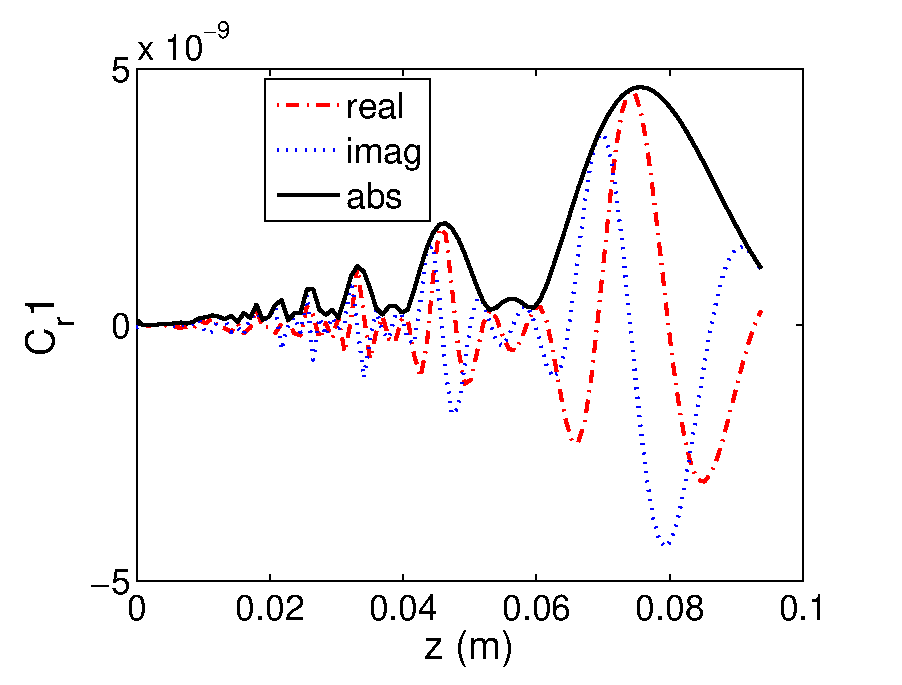
\includegraphics[scale=.44]{Figs/Cr1}}
\end{minipage}%
\begin{minipage}{.51\linewidth}
\centering
\subfloat[$ \mathcal{C}_{r_\perp}(z) $ for $ r_\perp > a $]{\label{Czb}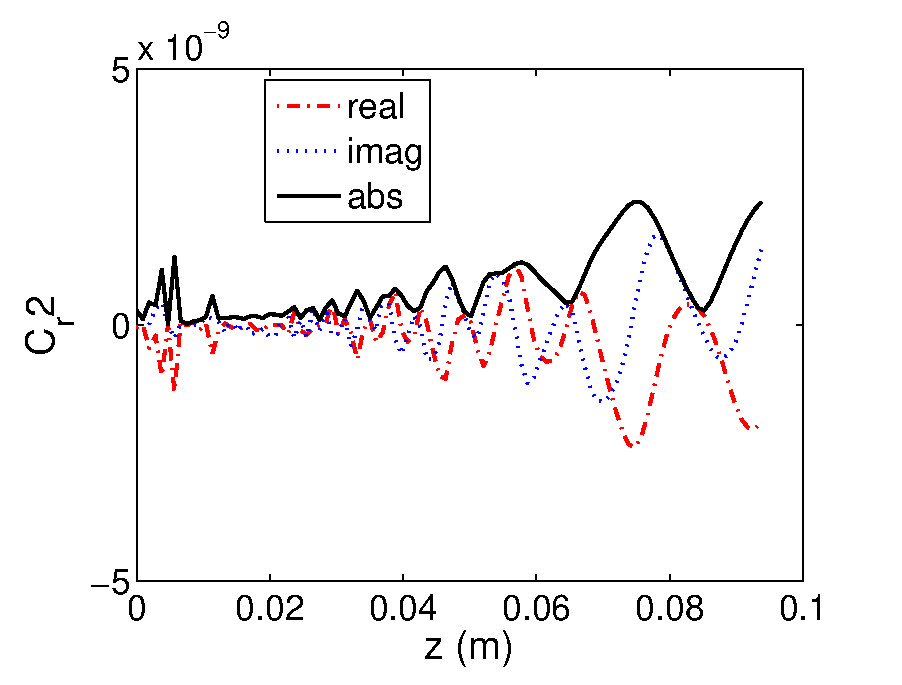
\includegraphics[scale=.44]{Figs/Cr2}}
\end{minipage}
\par\medskip
\begin{minipage}{.51\linewidth}
\centering
\subfloat[$ \mathcal{C}_\phi(z) $ for $ r_\perp < a $]{\label{Czc}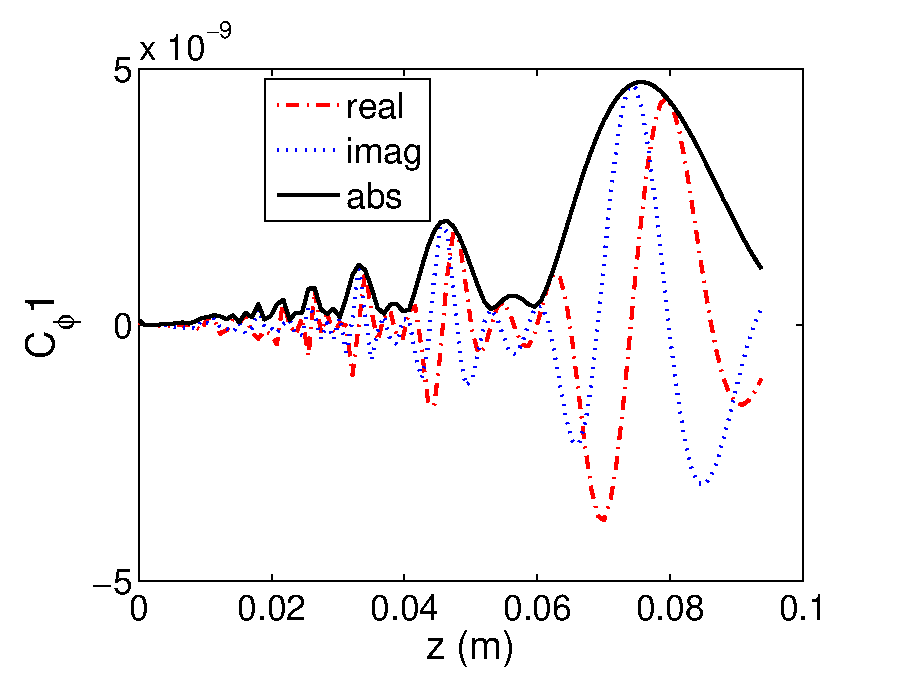
\includegraphics[scale=.44]{Figs/Cphi1}}
\end{minipage}%
\begin{minipage}{.51\linewidth}
\centering
\subfloat[$ \mathcal{C}_\phi(z) $ for $ r_\perp > a $]{\label{Czd}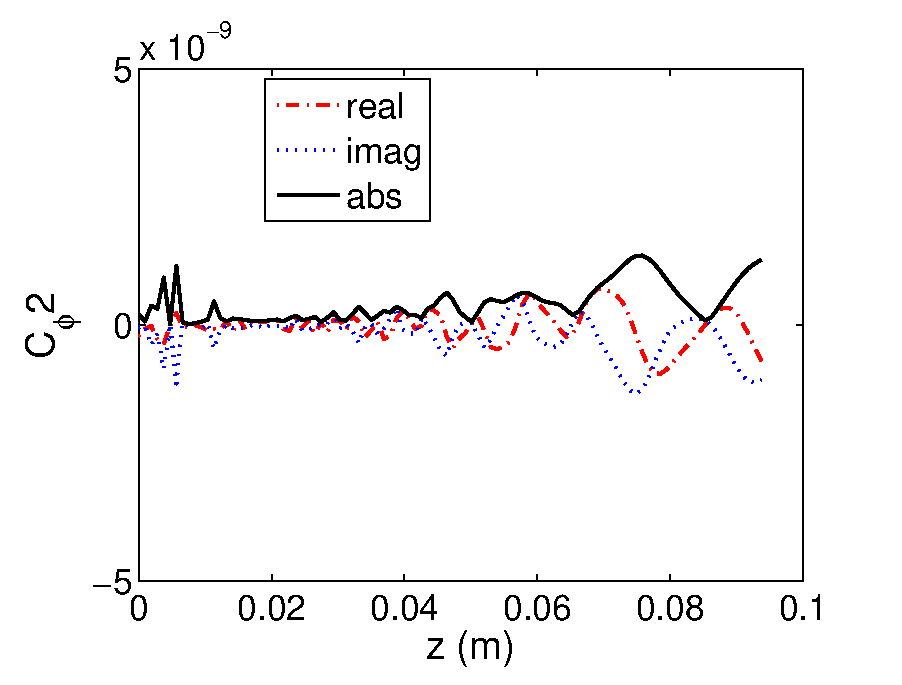
\includegraphics[scale=.44]{Figs/Cphi2}}
\end{minipage}
\caption{$ \mathcal{C}^{(\omega,p=+,f=+)}(z) $. The values of these coefficients are in an arbitrary unit. }
\label{Cz}
\end{figure}




\begin{figure}[H] 
\centering
\subfloat[$ \mathcal{A}(z) $]{\label{Az}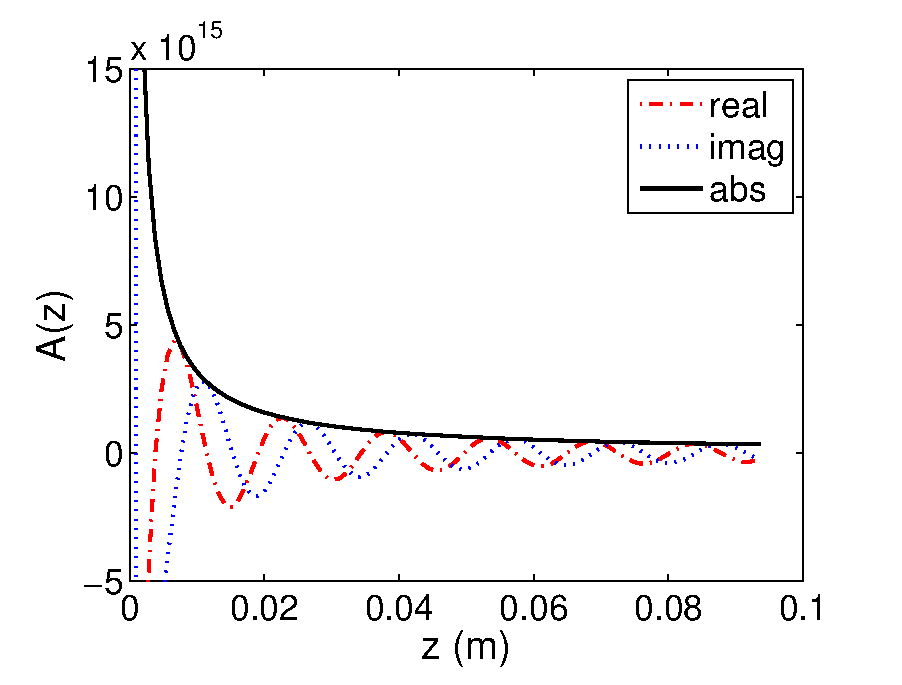
\includegraphics[scale=.5]{Figs/Az}}
\par\medskip
\begin{minipage}{.51\linewidth}
\centering
\subfloat[$ \mathcal{C}_{r_\perp}(z) $]{\label{Crz}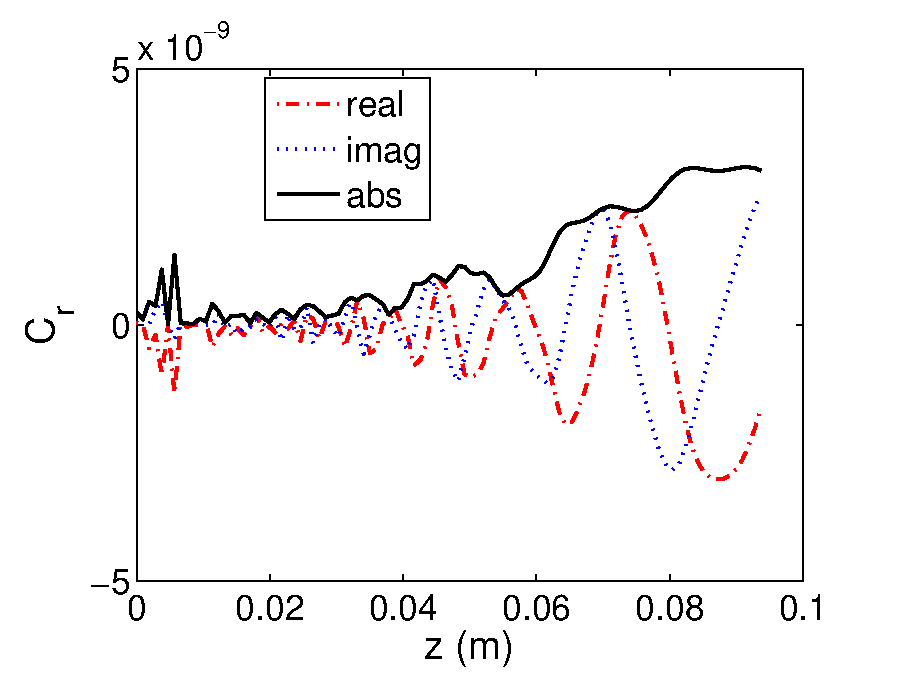
\includegraphics[scale=.44]{Figs/Cr}}
\end{minipage}%
\begin{minipage}{.51\linewidth}
\centering
\subfloat[$ \mathcal{C}_\phi(z) $ ]{\label{Cphiz}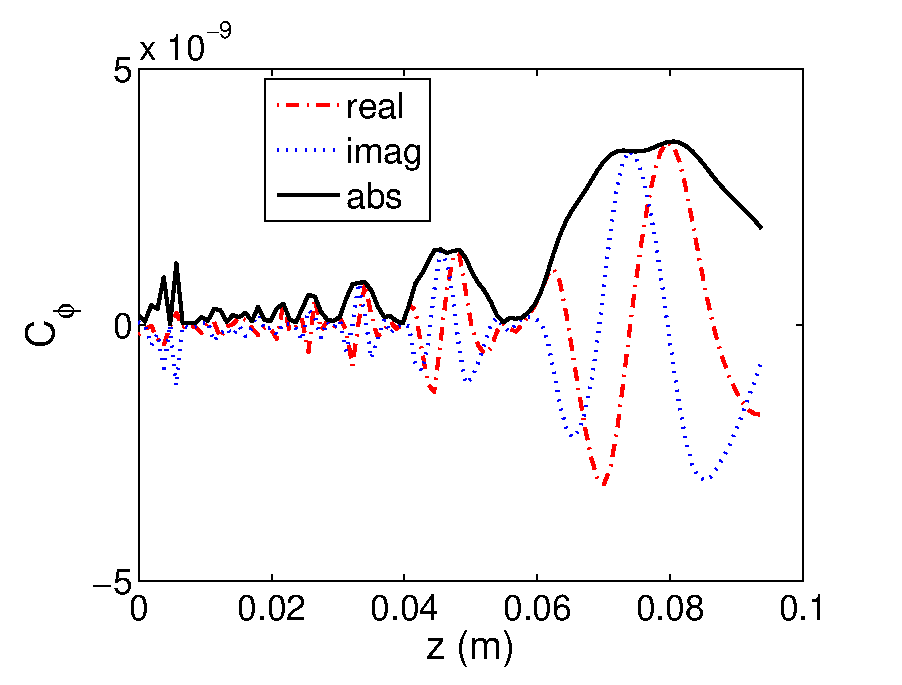
\includegraphics[scale=.44]{Figs/Cphi}}
\end{minipage}
\par\medskip
\begin{minipage}{.51\linewidth}
\centering
\subfloat[$ \mathcal{S}_{r_\perp}(z) $ ]{\label{Srz}\includegraphics[scale=.44]{Figs/Sr}}
\end{minipage}%
\begin{minipage}{.51\linewidth}
\centering
\subfloat[$ \mathcal{S}_\phi(z) $]{\label{Sphiz}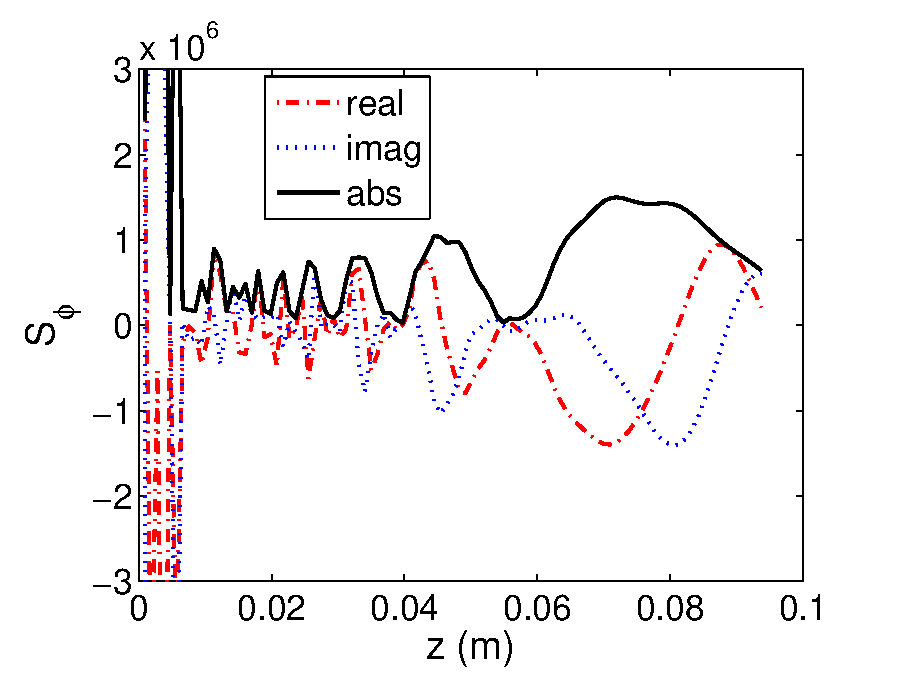
\includegraphics[scale=.44]{Figs/Sphi}}
\end{minipage}
\caption{$ \mathcal{A}(z) $, $ \mathcal{C}^{(\omega,p=+,f=+)}(z) $ and $ \mathcal{S}^{(\omega,p=+,f=+)}(z) $. The values of these coefficients are in an arbitrary unit. There should be some fast chopping in $ \mathcal{A}(z) $ and $ \mathcal{S}^{(\mu)}(z) $. However, due to the cost of computing time, we did not give a fine enough calculation in our plots. See following plots for the calculation results with an improved resolution.  }
\label{ACSz}
\end{figure}


\scalefig{Figs/InterferencePeriods}{0.6}{Wave path-difference of the interference between a monochromatic light emitted from a point atom located at $ \br'=(r'_\perp,\phi',z')=(2a,0,0) $ and a laser beam propagating along the $ z $-axis at the same wavelength $ \lambda_0=937.1 $ nm. The  horizontal axis of the plot is scaled in terms of the radium $ a $ of the nanofiber. The vertical axis is the wave path-difference measured along the laser's propagation direction of $ z $-axis, which is scaled by the wavelength $ \lambda=\lambda_0 $. As we can see, the interference period is uniform, and is on the order of $ 4.2a $.  This rough calculation implies that the chopping frequency in $ z $-direction should on the order of the wavelength, which should be reflected in Fig.~\ref{ACSz} and related plots. }


\newpage
Notice that, calculation resolution matters to the results. For comparison, we run the exact simulation as above but with a better $ z $-resolution.  The results are shown in Figs.~\ref{Cz_1} and~\ref{ACSz_1}. In $ z\in (0,1)\,\mathrm{mm} $ region, we calculate the coefficients in every $ 20 $ wavelengths; in $ z\in[2,100]\,\mathrm{mm} $ region, we calculate the coefficients in every $ \lesssim 1000 $ wavelengths. While in Figs.~\ref{Cz} and~\ref{ACSz} before, we calculate the coefficients evenly in every $ 1000 $ wavelengths. Also, when we calculated the integrals in the figures below, we used a $ 3 $ times better resolution in $ r_\perp\in(a,5a) $ region, which gives more detailed features of the $ \mathcal{C}^{(\mu)} (z)$ and $ \mathcal{S}^{(\mu)}(z) $ plots. With this improved resolution, it takes more than one hour to run the full calculation on a Thinkpad X200 laptop. 

\begin{figure}[H] 
\begin{minipage}{.51\linewidth}
\centering
\subfloat[$ \mathcal{C}_{r_\perp}(z) $ for $ r_\perp < a $]{\label{Cza_1}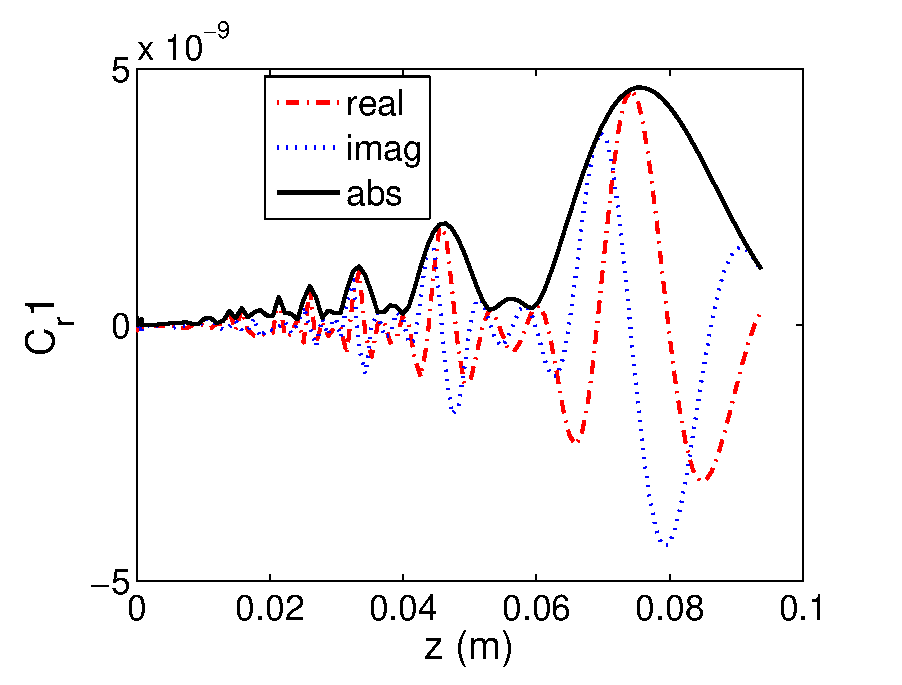
\includegraphics[scale=.44]{Figs/Cr1_1}}
\end{minipage}%
\begin{minipage}{.51\linewidth}
\centering
\subfloat[$ \mathcal{C}_{r_\perp}(z) $ for $ r_\perp > a $]{\label{Czb_1}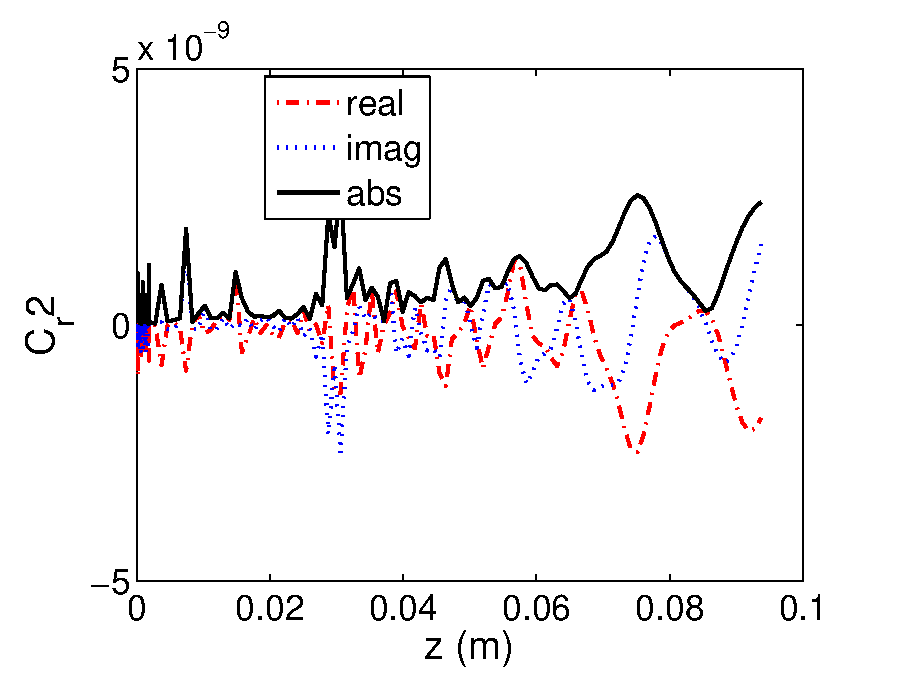
\includegraphics[scale=.44]{Figs/Cr2_1}}
\end{minipage}
\par\medskip
\begin{minipage}{.51\linewidth}
\centering
\subfloat[$ \mathcal{C}_\phi(z) $ for $ r_\perp < a $]{\label{Czc_1}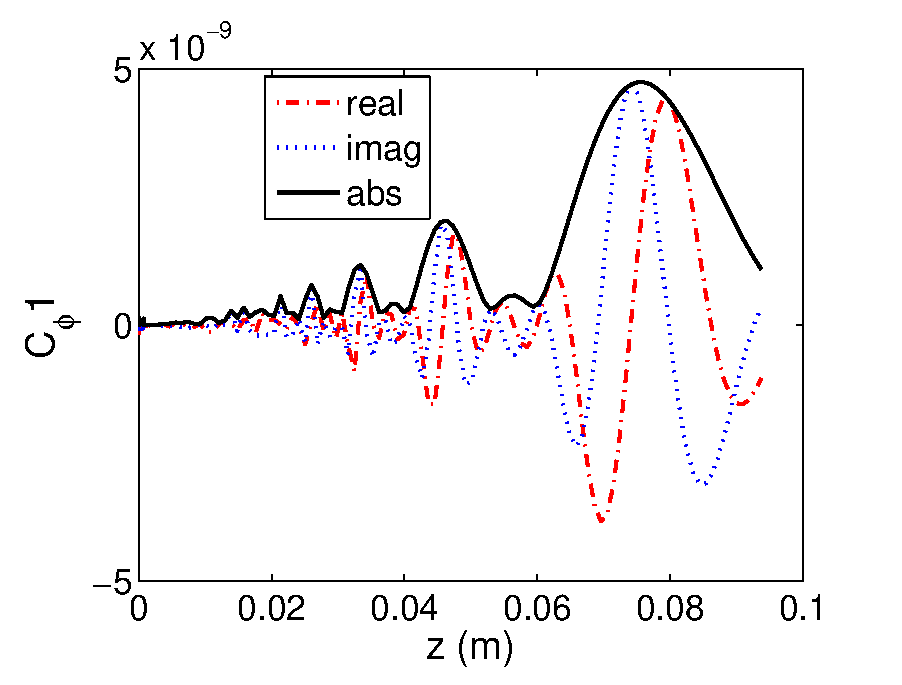
\includegraphics[scale=.44]{Figs/Cphi1_1}}
\end{minipage}%
\begin{minipage}{.51\linewidth}
\centering
\subfloat[$ \mathcal{C}_\phi(z) $ for $ r_\perp > a $]{\label{Czd_1}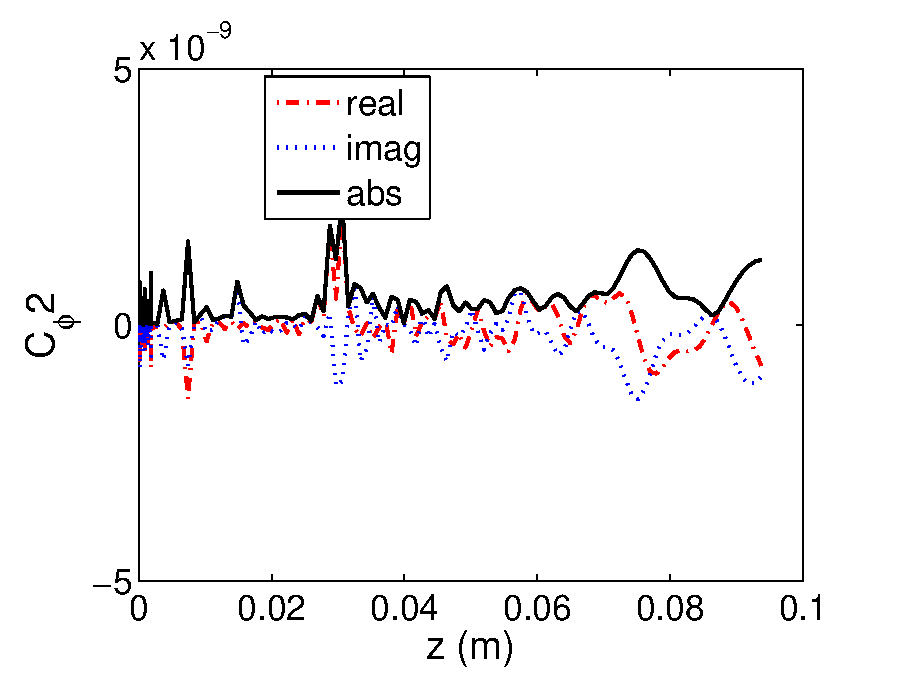
\includegraphics[scale=.44]{Figs/Cphi2_1}}
\end{minipage}
\caption{$ \mathcal{C}^{(\omega,p=+,f=+)}(z) $. The values of these coefficients are in an arbitrary unit. Resolution is improved (see text).}
\label{Cz_1}
\end{figure}




\begin{figure}[H] 
\centering
\subfloat[$ \mathcal{A}(z) $]{\label{Az_1}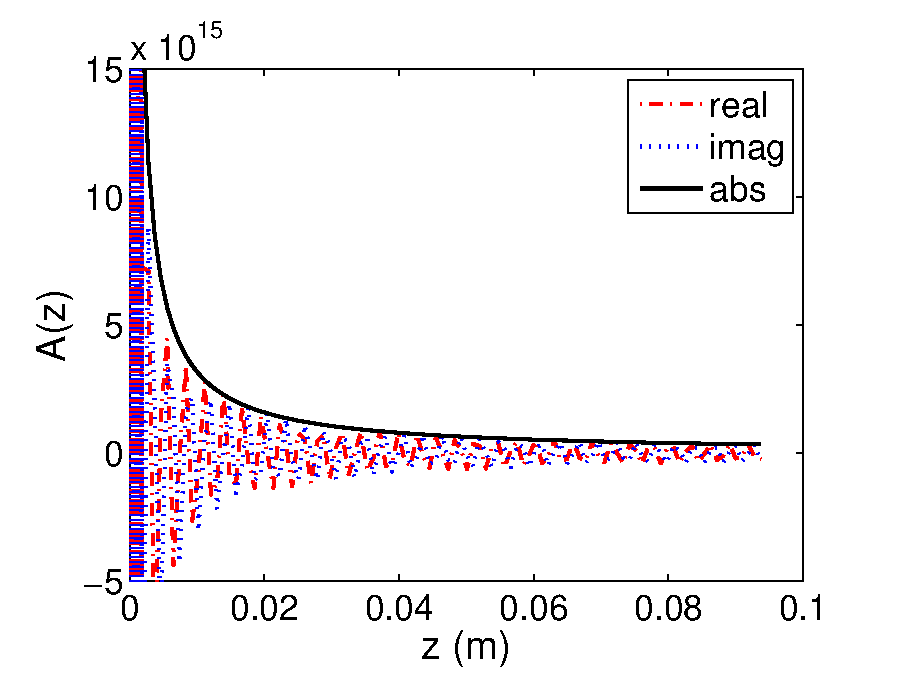
\includegraphics[scale=.5]{Figs/Az_1}}
\par\medskip
\begin{minipage}{.51\linewidth}
\centering
\subfloat[$ \mathcal{C}_{r_\perp}(z) $]{\label{Crz_1}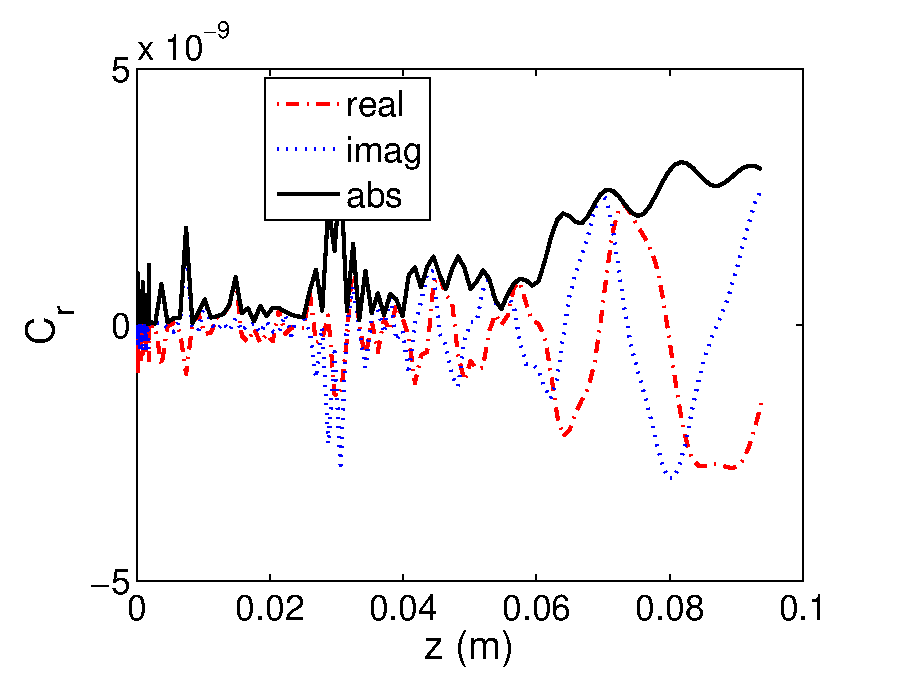
\includegraphics[scale=.44]{Figs/Cr_1}}
\end{minipage}%
\begin{minipage}{.51\linewidth}
\centering
\subfloat[$ \mathcal{C}_\phi(z) $ ]{\label{Cphiz_1}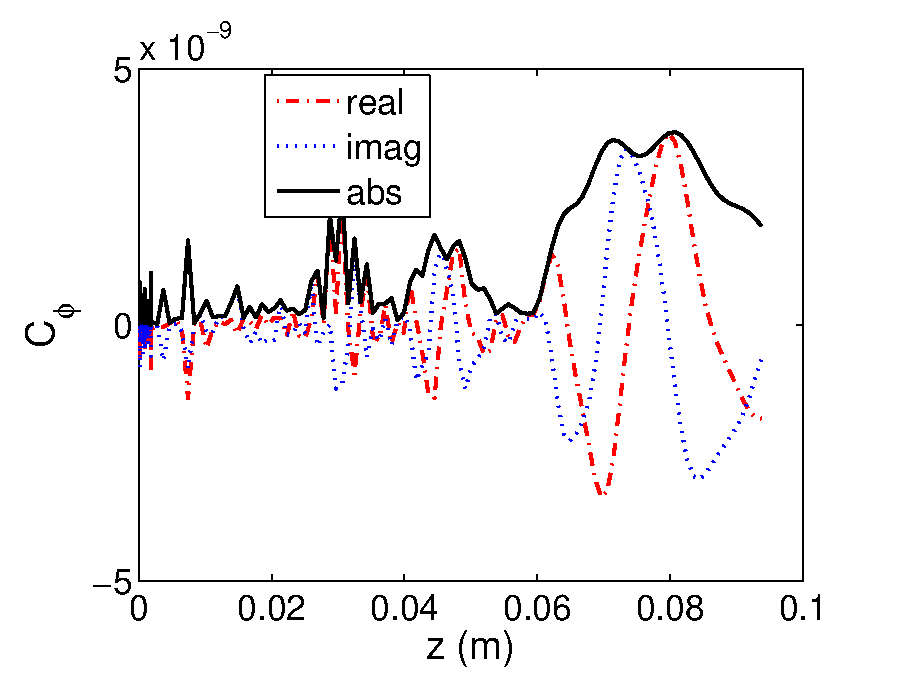
\includegraphics[scale=.44]{Figs/Cphi_1}}
\end{minipage}
\par\medskip
\begin{minipage}{.51\linewidth}
\centering
\subfloat[$ \mathcal{S}_{r_\perp}(z) $ ]{\label{Srz_1}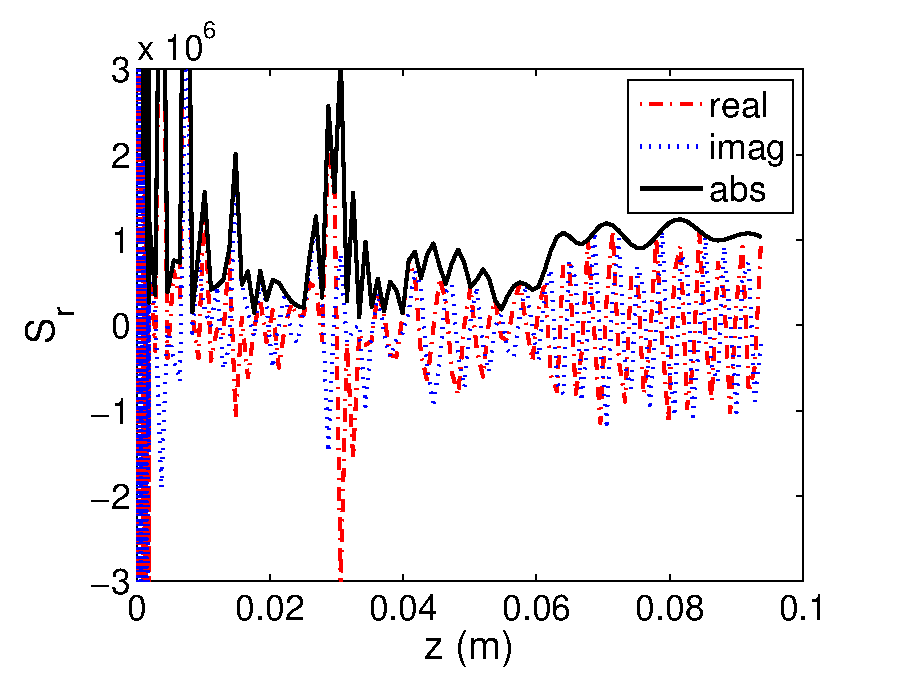
\includegraphics[scale=.44]{Figs/Sr_1}}
\end{minipage}%
\begin{minipage}{.51\linewidth}
\centering
\subfloat[$ \mathcal{S}_\phi(z) $]{\label{Sphiz_1}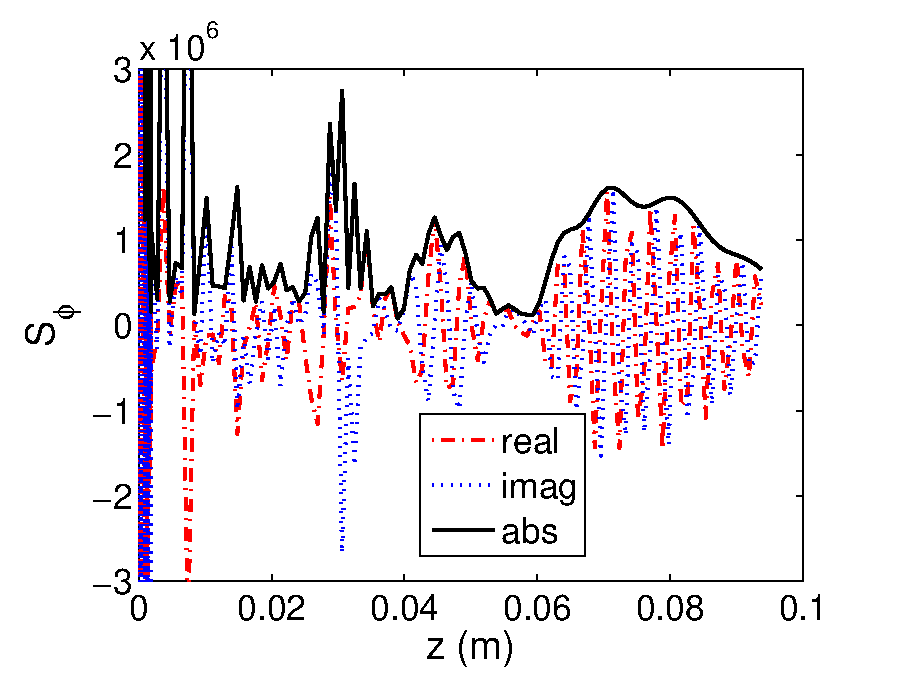
\includegraphics[scale=.44]{Figs/Sphi_1}}
\end{minipage}
\caption{$ \mathcal{A}(z) $, $ \mathcal{C}^{(\omega,p=+,f=+)}(z) $ and $ \mathcal{S}^{(\omega,p=+,f=+)}(z) $. The values of these coefficients are in an arbitrary unit. Resolution is improved (see text).}
\label{ACSz_1}
\end{figure}


\section{Bound and radiation modes}
In our study, it is critical to separate the bound mode and the radiation mode. In this section, we will 
go through a light propagation theory in the scenario of a nanofiber with a trapped atom. 

Considering that the atom emits photons around the nanofiber, the total electrical field in our problem 
can be written as 
\begin{align}\label{Esrt0}
\boldsymbol{\mathcal{E}}(\br) = \boldsymbol{\mathcal{E}}_{source}(\br) + 
\boldsymbol{\mathcal{E}}_{fiber}(\br)=\boldsymbol{\mathcal{E}}_{source}(\br) + 
\boldsymbol{\mathcal{E}}_{ref}(\br) +\boldsymbol{\mathcal{E}}_{tran}(\br),
\end{align}
where $ \boldsymbol{\mathcal{E}}_{source} $ is the electrical field generated by the atom source;  $ 
\boldsymbol{\mathcal{E}}_{fiber} $ is the field due to the presence of the nanofiber, which includes the 
reflected electrical field $ \boldsymbol{\mathcal{E}}_{ref}(\br) $ (outside the nanofiber) and transmitted field $ 
\boldsymbol{\mathcal{E}}_{tran}(\br) $ (inside the nanofiber). 

First, we only consider the light propagating in a nanofiber without any scatterers. We estimate 
the field propagating along the nanofiber is a cylindrical wave due to the geometrical symmetry of the 
nanofiber. 

To fully calculate the electromagnetic field, we consider both electrical and magnetic fields, the spacial 
parts of which are governed by the wave equations
\begin{align}\label{EBz}
\left(\nabla^2 +k^2 \varepsilon(\br_{\perp})\right) \begin{pmatrix}
\mathcal{E}_z(\br)\\
\mathcal{B}_z(\br)
\end{pmatrix} = 0.
\end{align}
Notice that we are working in the cylindrical coordinate system, and only concentrate on the $ z 
$-component of the fields, since all the other components can be expressed in terms of the $ z 
$-components of the fields (see Appendix \ref{MWE:components}. It will be discussed shortly). 

We use an ansatz that 
\begin{align}
\mathcal{E}_z (r_\perp, \phi, z) &= \psi(r_\perp,\phi) e^{i\beta z}\\
\mathcal{B}_z (r_\perp,\phi,z) &= \zeta(r_\perp,\phi) e^{i\beta z}.
\end{align}
Substituting the above into Equ.~\ref{EBz}, we obtain
\begin{align}\label{psizeta}
\left(\nabla^2_\perp +(k^2 \varepsilon(\br_{\perp})-\beta^2 )\right) \begin{pmatrix}
\psi(r_\perp,\phi)\\
\zeta(r_\perp,\phi)
\end{pmatrix} = 0.
\end{align}
Now, the problem of solving a three dimensional wave equation for $ \mathcal{E} (r_\perp, \phi, z) $ 
and $ \mathcal{B} (r_\perp, \phi, z)$ turns into a problem of solving a two dimensional differential 
(mode) equation for $ \psi(r_\perp,\phi) $ and $ \zeta(r_\perp,\phi) $. 

There are two special cases for the modes, in general. If $ \psi=0 $ as a constant, which means there is 
no $ z $-component of the electrical field, then the propagating mode is call a TE mode\index{mode!TE 
mode}. Similarly, if $ \zeta=0 $ as a constant, which corresponds to zero magnetic $ z $-component, 
then this mode is called a TM mode\index{mode!TM mode}. However, the modes in a waveguide with 
cylindrical symmetry cannot be grouped into TE and TM guided waves. In general, the modes with 
both electrical and magnetic nonzero $ z $-components are known as EH and HE hybrid 
modes\index{mode!HE mode}~\cite{Snyder1983}.

We focus on the electrical part for now. The magnetic field can be solved similarly. Equ.~\ref{psizeta} 
gives
\begin{align}\label{eigenpsi}
[\nabla^2_\perp + k^2\varepsilon(r_\perp)] \psi(r_\perp, \phi) = \beta^2\psi(r_\perp,\phi).
\end{align}
Compared to the time-independent Schrodinger equation
\begin{align}
\left[\frac{\hat{P}^2}{2m}+V(\hat{\mathbf{r}}_\perp) \right] \psi(\br_\perp)&= E\psi(\br_\perp)\\
\text{or}\quad \left[ \nabla^2_\perp -V(r_\perp) \right] \psi (r_\perp, \phi) &= -E\psi(r_\perp,\phi),
\end{align}
we can conclude that the mode equation (Equ.~\ref{eigenpsi}) is basically an eigenvalue equation if we 
make 
\begin{align}
V_{ef\!f}=-k^2\varepsilon(\br\!_\perp) &\sim V(\br\!_\perp)\\
-\beta^2 &\sim E.
\end{align}
With these analogies, we can apply the method of distinguishing bound and unbound or radiative wave 
functions we used in the time-independent Schrodinger equation to distinguishing the bound and 
radiation modes in our nanofiber model. 

In the time-independent Schrodinger problem, if $ 0<E\leq V $, then the wave is bounded; if $ E>V $, 
then the wave is unbounded. For the fiber mode, similarly, we can also use the relative position of $ 
V_{ef\!f} $ and $ -\beta^2 $ to classify the bound and radiation modes (see 
Fig.~\ref{Figs/scatteredmode}).

\scalefig{Figs/scatteredmode}{0.8}{Bound and unbound states for the nanofiber eigenvalue 
problem. $ \varepsilon(r\!_\perp)=\varepsilon_{f} =n_1^2$ if $ r_\perp < a $; otherwise, $\varepsilon
(r\!_\perp) =1 $. The parameter $ a $ is the radium of the nanofiber. } 

Using the relationship that
\begin{align}
\nabla^2 \!_\perp = \frac{1}{r_{\!\perp}}\pp{}{r\!_\perp}\! \left(r\!_\perp \pp{}{r\!_\perp} \right) + 
\frac{1}{r_\perp^2} \spp{}{\phi},
\end{align}
and the symmetry of the fiber,  we can  separate the mode function by
\begin{align}
\psi(r\!_\perp,\phi)=\mathcal{E}_{z,\beta m}(r\!_\perp)e^{im\phi},
\end{align} 
and hence
\begin{align}
\mathcal{E}_z(r\!_\perp,\phi,z) = \mathcal{E}_{z,\beta m}(r\!_\perp)e^{i(m\phi+\beta z)},
\end{align}
where $ \mathcal{E}_{z,\beta m}(r\!_\perp) $ satisfies the Bessel's equation
\begin{align}
\left[ \spp{}{r\!_\perp}+ \frac{1}{r_{\!\perp}}\pp{}{r\!_\perp}- 
\frac{m^2}{r^2\!_\perp} + (k^2\varepsilon(r\!_\perp)-\beta^2) \right] 
\mathcal{E}_{z,\beta m}(r\!\!_\perp)=0
\end{align}
with 
\begin{align}
\varepsilon(r\!\!_\perp) = 
\begin{cases}
1, & r\!_\perp>a\\
\varepsilon_f, & r\!_\perp\leq a.
\end{cases}
\end{align}
The general solution for $ \mathcal{E}_{z,\beta m}(r\!\!_\perp) $ can be given in three cases 
corresponding to different 
boundary conditions
\begin{align}
\mathcal{E}_{z,\beta m}(r\!\!_\perp) = \begin{cases}
AJ_m(qr\!\!_\perp) + B Y_m(qr\!_\perp)&\rightarrow J_m(\theta)\sim \cos\theta,\, Y_m(\theta)\sim 
\sin\theta.\\
CI_m(qr\!_\perp) + DK_m(qr\!_\perp) & \rightarrow I_m(\theta) \sim e^\theta,\, K_m(\theta) \sim 
e^{-\theta}.\\
EH_m^{(\!1\!)}(qr\!_\perp) \!+\! FH_m^{(\!2\!)}(qr\!_\perp ) & \rightarrow H_m^{(\!1\!)} (\theta) \! \sim \! 
e^{i\theta},\, 
H_m^{(\!2\!)}(\theta)\!\sim\! e^{\!-i\theta}.
\end{cases}
\end{align}
The positive parameter $ 1/q $ is the characteristic decay length corresponding to $ 1/h_{11} $ and $ 
1/q_{11} $ 
in the $\text{HE}_{11}$ mode expression. Using the symmetric and convergent condition at $ 
r\!_\perp=0\,\text{and}\, \infty $, as for bound modes, for example, if $k< \beta\leq 
k\sqrt{\varepsilon_f}$,
\begin{align}
\left\{
 \begin{array}{lcll}
	r\!_\perp \leq a, & \mathcal{E}_{z,\beta m}(r\!_\perp )\!=\! AJ_m(h r\!_\perp), & h \!=\! 
	\sqrt{k^2\varepsilon_f-\beta^2}\! >\! 0;\\
	r\!_\perp > a, & \mathcal{E}_{z,\beta m}(r\!_\perp )\!=\!DK_m(q r\!_\perp), & q\!=\! 
	\sqrt{\beta^2-k^2}>0.
 \end{array}\right.
\end{align}
Both $ \beta $ and $ h $ are discrete for bound modes. 
For scattered modes, $ 0\leq \beta< k $, similarly, 
\begin{align}
\left\{
 \begin{array}{lcll}
	r\!_\perp \leq a, & \mathcal{E}_{z,\beta m}(r\!_\perp )\!=\! AJ_m(h r\!_\perp), & h \!=\! 
	\sqrt{k^2\varepsilon_f-\beta^2}\! >\! 0;\\
	r\!_\perp > a, & \mathcal{E}_{z,\beta m}(r\!_\perp )\!=\!EH_m^{(\!1\!)}(p r\!_\perp\!), & p\!\!=\!\! 
	\sqrt{k^2-\beta^2}>0.
 \end{array}\right.
\end{align}
Both $ \beta $ and $ p $ are continuous. \textcolor{red}{(Double check the general solutions and the consistence with Equ.~\ref{ET0Rexpand}.)}
%Notice that Ref.\cite{Snyder1983} used $ J_m(hr\!_\perp)\cos m\phi $ and $ 
%(J_m(pr\!_\perp)+CH_m^{(\!1\!)})\cos m\phi $ as the basis for the general solution of $ e $ and $ o $ 
%light 
%of the radiation modes, and summed them up. They are equivalent to the solution here.  

If $ \beta $ is a pure imaginary number, the field will have an exponential decay amplitude on $ z $-direction, and will spread the energy away from the fiber axis. Reference~\cite{Snyder1983} denotes the modes with pure imaginary $ \beta $ as evanescent modes. If $ \beta $ has both real and imaginary parts, the modes are denoted as leaky modes, which are combinations of radiation modes and evanescent modes. Except for the case that the incident light is highly directed at the complementary critical angle $ \theta_c $ of geometric optics, only the radiation modes part can propagate for a long distance along the fiber axis. In our nanofiber system, we only consider the bound and radiation modes. The ranges of some waveguide parameters are given in Table~\ref{tab:fiberparameters}. 
In the table, we have defined the normalized wave number\cite{Snyder1983}, or 
$V$-number\index{$V$-number} 
of a fiber as $V  = 
k_f a \mathrm{NA}$.  Here $k_f=\frac{2\pi}{\lambda}$, is the free space wave number, $a$ is the radius 
of the core of the fiber, and $\mathrm{NA}$ is the numerical aperture\index{numerical aperture} of 
the fiber, $\mathrm{NA} = 
(n_{core}^2 - n_{cladding}^2)^{1/2} = n_{core}(2\Delta)^{1/2}$, with profile height 
parameter\index{profile height parameter} 
$\Delta =\frac{1}{2}(1-n_{cladding}^2/n_{core}^2)\approx (n_{core}-n_{cladding})/n_{core}$.  For 
different modes labeled with $ j $, we always have $V_j^2=a^2(h_j^2+q_j^2)$ and $ \lambda\beta_j/2\pi $ is a mode invariance.  The TE and TM modes have non-vanishing cut-off 
frequencies, as $ a\rightarrow 0 $.  The cutoff frequency is found from $V = a\omega (\Delta)^{1/2}/c =2.405$ for silicon fiber.  
Only the lowest HE mode, $\mathrm{HE}_{11}$, has no cutoff frequency as $ a\rightarrow 0 $.  For $0 < V < 2.405$, which is the case of the nanofiber we are studying, it is the only mode that propagates in the 
fiber. For fixed $ \varepsilon_f $, in the range that $ 0\leq \beta \leq 
k\sqrt{\varepsilon_f} $, we can distinguish the radiative and bound mode as follows:
\begin{align}
\begin{cases}
0\leq \beta < k, &\rightarrow \textit{unbounded radiative modes;}\\
k< \beta \leq k \sqrt{\varepsilon_f}, &\rightarrow \exists a,\, \textit{HE}_{11}\, \textit{is the only 
bound mode.}
\end{cases}
\end{align}


\begin{minipage}{\linewidth}
\centering
\captionof{table}{Ranges of fiber parameters for basic modes. Superscripts $ r $ and $ i $ denote real and imaginary parts. Subscripts $ j $ denotes the discrete values for bound modes. Adapted from Ref.\cite{Snyder1983} P.P.516 Table 25-1.} \label{tab:fiberparameters} 
\begin{tabular}{|l|c|c|c|}
\hline  & $\beta$ & $h$ & $p$ \\ 
\hline Bound modes & $k<\beta_j \leq k\sqrt{\varepsilon_f} $ & $ 0\leq h_j<V/a $ & $ p^r_j=0,\, p^i_j>0 $ \\ 
\hline Radiation modes & $0\leq \beta<k$ & $V/a < h\leq k\sqrt{\varepsilon_f}$ & $0<p\leq k $\\ 
\hline Evanescent modes & $ \beta^r=0,\, \beta^i>0 $ & $ k\sqrt{\varepsilon_f} < h $ & $ k<p $ \\ 
\hline 
\end{tabular} 
\par
\bigskip
%Should be a caption
\end{minipage}

Due to the symmetry of equations, we also have
\begin{align}
\mathcal{B}_z(r\!_\perp,\phi,z) = \mathcal{B}_{z,\beta m}(r\!_\perp)e^{i(m\phi+\beta z)},
\end{align}
where $  \mathcal{B}_{z,\beta m}(r\!_\perp) $ satisfies the same Bessel's equation as above. 

Next, we consider the case that an atom--which can be treated as a dipole--is placed next to the 
nanofiber. Equ.~\ref{Esrt0} can be rewritten as 
\begin{align}
\boldsymbol{\mathcal{E}}(\br) &= \boldsymbol{\mathcal{E}}_{source}(\br) + 
\boldsymbol{\mathcal{E}}_{ref}(\br)+\boldsymbol{\mathcal{E}}_{tran}(\br)\\
&=
	\begin{cases}
	  \boldsymbol{\mathcal{E}}_{dipole} (\br)+ \boldsymbol{\mathcal{E}}_{ref}(\br) & r\!_\perp \geq a,\\
	  \boldsymbol{\mathcal{E}}_{tran}(\br) & r\!_\perp<a.
	\end{cases} \label{Etotalfiber}
\end{align}


For longitudinal components of the electrical and magnetic fields we expand them as follows
\begin{subequations}\label{ET0Rexpand}
\begin{align}
\mathcal{E}^{(T)}_z &= \sum_{m=-\infty}^\infty \int \mathrm{d}\beta e^{im(\phi-\phi') + i\beta (z-z')} \mathcal{E}^{(T)}_{z,m\beta}(r\!_\perp)\\
&= \sum_{m=-\infty}^\infty \int \mathrm{d}\beta e^{im(\phi-\phi') + i\beta (z-z')} c_{m\beta} J_m (hr\!_\perp),\\
% + B_{m\beta} Y_m(hr\!_\perp)\right],\\
\mathcal{E}^{(0)}_{z} &= \sum_{m=-\infty}^\infty \int \mathrm{d}\beta e^{im(\phi-\phi') + i\beta (z-z')} \mathcal{E}^{(0)}_{z,m\beta}(r\!_\perp)\\
\mathcal{E}^{(R)}_z &= \sum_{m=-\infty}^\infty \int \mathrm{d}\beta e^{im(\phi-\phi') + i\beta (z-z')} \mathcal{E}^{(R)}_{z,m\beta}(r\!_\perp)\\
&= \sum_{m=-\infty}^\infty \int \mathrm{d}\beta e^{im(\phi-\phi') + i\beta (z-z')} a_{m\beta} H_m^{(1)} (pr\!_\perp),
\end{align}
\end{subequations}
\begin{subequations}\label{BT0Rexpand}
\begin{align}
\mathcal{B}^{(T)}_z &= \sum_{m=-\infty}^\infty \int \mathrm{d}\beta e^{im(\phi-\phi') + i\beta (z-z')} \mathcal{B}^{(T)}_{z,m\beta}(r\!_\perp)\\
&= \sum_{m=-\infty}^\infty \int \mathrm{d}\beta e^{im(\phi-\phi') + i\beta (z-z')} d_{m\beta} J_m (hr\!_\perp),\\
% + E_{m\beta} Y_m(hr\!_\perp)\right],\\
\mathcal{B}^{(0)}_{z} &= \sum_{m=-\infty}^\infty \int \mathrm{d}\beta e^{im(\phi-\phi') + i\beta (z-z')} \mathcal{B}^{(0)}_{z,m\beta}(r\!_\perp)\\
\mathcal{B}^{(R)}_z &= \sum_{m=-\infty}^\infty \int \mathrm{d}\beta e^{im(\phi-\phi') + i\beta (z-z')} \mathcal{B}^{(R)}_{z,m\beta}(r\!_\perp)\\
&= \sum_{m=-\infty}^\infty \int \mathrm{d}\beta e^{im(\phi-\phi') + i\beta (z-z')} b_{m\beta} H_m^{(1)} (pr\!_\perp),
\end{align}
\end{subequations}
where the subscripts indicate the field components of reflection ($R$), dipole oscillation in free space ($0$) and transmission ($ T $). Notice that we have chosen $ m=\pm 1 $, as the nanofiber can only support HE$_{11}$ modes. 
The $ r\!_\perp $ and $ \phi $ components of the fields can be obtained using Equ.~\ref{EHzgauss} and $ \mathcal{B}=\mathcal{H} $ in Gauss units for given $ m $. \textcolor{red}{Also notice, whether we should use $ e^{im\phi + i\beta z} $ or $ e^{im(\phi-\phi') + i\beta (z-z')} $ in the equations above is not clear. Using $ e^{im(\phi-\phi') + i\beta (z-z')} $ is more convenient to solve the boundary condition problem, but Klimov's paper uses the other one. See the discussion on boundary conditions next.}

The free space dipole emits an electromagnetic field described by
\begin{align}
\mathcal{A} &= -ik \mathbf{d}_0 \frac{e^{ik|\br-\br'|}}{|\br-\br'|},
\end{align}
\begin{align}
\mathcal{B} &= \nabla\times \mathcal{A}\nonumber \\
&=(\frac{1}{r\!_\perp}\pp{A_z}{\phi}-\pp{A_\phi}{z})\mathbf{e}_{r\!_{\perp}}+(\pp{A_{r\!_\perp}}{z}-\pp{A_z}{r\!_\perp})\mathbf{e}_\phi + \frac{1}{r\!_\perp}(\pp{(r\!_\perp A_\phi)}{r\!_\perp}-\pp{A_{r\!_\perp}}{\phi})\mathbf{e}_z,\\
\mathcal{E} &= \frac{i}{k} \nabla\times \mathcal{H}=\frac{i}{k}\nabla\times \mathcal{B},
\end{align}
or, by Equ.~\ref{EGd}. Here, $ \mathbf{d}_0 $ is the dipole momentum in vacuum. where ${\rm {\bf r}}=\left( {r\!_\perp ,\phi ,z}\right) $ and ${\rm 
{\bf {r}^{\prime }}}=\left( {{r\!_\perp }^{\prime },{\phi }^{\prime },{z}%
^{\prime }}\right) $ are radius vectors of observation point and atom
position. Using the expansion for the space $ \left(r\!_\perp <r_\perp ^{\prime}\right) $ that 
\begin{align}
{\frac{{e^{ik{\left| {{\rm {\bf r}}-{\rm {\bf {r}^{\prime }}}}\right| }}}}{{{%
\left| {{\rm {\bf r}}-{\rm {\bf {r}^{\prime }}}}\right| }}}}
={\frac{{i}}{{2}}%
}{\sum\limits_{m=-\infty }^{\infty } {{\oint\limits_{C_{1}}{\mathrm{d}\beta \;e^{im\left( {\phi -{\phi }%
^{\prime }}\right) +i\beta \left( {z-{z}^{\prime }}\right) }J_{m}\left( {pr\!_\perp
}\right) H_{m}^{\left( {1}\right) }\left( pr_\perp ^{\prime
}\right) }}}},
\end{align}
and for $ \left(r\!_\perp >r_\perp ^{\prime}\right) $
\begin{align}
{\frac{{e^{ik{\left| {{\rm {\bf r}}-{\rm {\bf {r}^{\prime }}}}\right| }}}}{{{%
\left| {{\rm {\bf r}}-{\rm {\bf {r}^{\prime }}}}\right| }}}}
={\frac{{i}}{{2}}%
}{\sum\limits_{m=-\infty }^{\infty } {{\oint\limits_{C_{1}}{\mathrm{d}\beta \;e^{im\left( {\phi -{\phi }%
^{\prime }}\right) +i\beta \left( {z-{z}^{\prime }}\right) }J_{m}\left( {pr\!_\perp^{\prime} }\right) H_{m}^{\left( {1}\right) }\left( pr_\perp \right) }}}},
\end{align}
one can obtain the free space dipole radiation field components in Equ.~\ref{ET0Rexpand} and~\ref{BT0Rexpand}. The contour $ C_1 $ and field components can be found in Ref.~\cite{Klimov2004}. Below, we present the field components that the reference did not include for the case of $ r\!_\perp>r'\!_\perp $ \textcolor{red}{(also, if we exchange $ J_m $ and $ H^{(1)}_m $ functions below, the result should recover the result for $ r\!_\perp<r'\!_\perp $ case. By comparing the result with Klimov's paper for the $ r\!_\perp<r'\!_\perp $ case, it seems Klimov has used some tricks, because there are some derivatives with respect to $r\!_\perp$ in the paper which can be either obtained from the factor $  e^{im\phi' + i\beta z'}  $ that we announced earlier or from some symmetry of the Bessel functions. The boundary condition solution is to be double checked.)}. The magnetic field components for $ \br\!_\perp>\br'\!_\perp $ are 
\begin{align}
\mathcal{B}_{z,m\beta}^{(0)} &= \frac{k}{2r\!_\perp}\left[(d^0_\phi\!-\! id^0_{r\!_\perp}m) J_m(pr'\!\!_\perp)H_m^{(1)}(pr\!_\perp) \!+\! d^0_\phi r\!_\perp J_m(pr'\!_\perp) \frac{\mathrm{d}}{\mathrm{d}r\!_\perp}H_m^{(1)}(pr\!_\perp)\right]\\
\mathcal{B}_{\phi,m\beta}^{(0)} &= \frac{k}{2}\left[ id^0_{r\!_\perp}\beta J_{m}\left( {pr\!_\perp^{\prime} }\right) H_{m}^{\left( {1}\right) }\left( pr\!_\perp \right)-d^0_z J_{m}\left( {pr\!_\perp^{\prime} }\right) \frac{\mathrm{d}}{\mathrm{d}r\!_\perp}H_{m}^{\left( {1}\right) }\left( pr\!_\perp \right) \right]\\
\mathcal{B}_{r\!_\perp, m\beta}^{(0)} &= \frac{k}{2}\left[(\frac{id^0_z m}{r\!_\perp}- id^0_\phi \beta)J_{m}\left( {pr\!_\perp^{\prime} }\right) H_{m}^{\left( {1}\right) }\left( pr\!_\perp \right)   \right]\\
\mathcal{E}_{z,m\beta}^{(0)} &= \frac{1}{r\!_\perp}\left[\frac{k}{2}\left[ id^0_{r\!_\perp}\beta J_{m}\left( {pr\!_\perp^{\prime} }\right) H_{m}^{\left( {1}\right) }\left( pr\!_\perp \right)-d^0_z J_{m}\left( {pr\!_\perp^{\prime} }\right) \frac{\mathrm{d}}{\mathrm{d}r\!_\perp}H_{m}^{\left( {1}\right) }\left( pr\!_\perp \right) \right]\right.\nonumber\\
&\qquad + \frac{kr\!_\perp}{2}\left[ id^0_{r\!_\perp}\beta J_{m}\left( {pr\!_\perp^{\prime} }\right) \frac{\mathrm{d}}{\mathrm{d}r\!_\perp}H_{m}^{\left( {1}\right) }\left( pr\!_\perp \right)-d^0_z J_{m}\left( {pr\!_\perp^{\prime} }\right) \frac{\mathrm{d}^2}{\mathrm{d}r^2\!\!_\perp}H_{m}^{\left( {1}\right) }\left( pr\!_\perp \right) \right] \nonumber\\
&\qquad -\left. \frac{imk}{2}(\frac{id^0_z m}{r\!_\perp}- id^0_\phi \beta)J_{m}\left( {pr\!_\perp^{\prime} }\right) H_{m}^{\left( {1}\right) }\left( pr\!_\perp \right)  \right]\\
&= \frac{k}{2r\!_\perp}\left[ (\dfrac{d^0_z m^2}{r\!_\perp}-d^0_\phi m \beta + i d^0_{r\!_\perp}\beta)J_{m}\left( {pr\!_\perp^{\prime} }\right) H_{m}^{\left( {1}\right) }\left( pr\!_\perp \right)\right. \nonumber \\
&\qquad\qquad +(id^0_{r\!_\perp}\beta r\!_\perp -d^0_z)J_{m}\left( {pr\!_\perp^{\prime} }\right) \frac{\mathrm{d}}{\mathrm{d}r\!_\perp}H_{m}^{\left( {1}\right) }\left( pr\!_\perp \right)\nonumber\\
&\qquad\qquad \left. - d^0_z r\!_\perp J_{m}\left( {pr\!_\perp^{\prime} }\right) \frac{\mathrm{d}^2}{\mathrm{d}r^2\!\!_\perp}H_{m}^{\left( {1}\right) }\left( pr\!_\perp \right) \right]\\
\mathcal{E}_{\phi,m\beta}^{(0)} &= \frac{ik\beta}{2}\left[ id^0_{r\!_\perp}\beta J_{m}\left( {pr\!_\perp^{\prime} }\right) H_{m}^{\left( {1}\right) }\left( pr_\perp \right)-d^0_z J_{m}\left( {pr\!_\perp^{\prime} }\right) \frac{\mathrm{d}}{\mathrm{d}r\!_\perp}H_{m}^{\left( {1}\right) }\left( pr_\perp \right) \right]\nonumber\\
&\quad +\frac{k}{2r^2\!\!_\perp}\left[(d^0_\phi\!-\! id^0_{r\!_\perp}m) J_m(pr'\!\!_\perp)H_m^{(1)}(pr\!_\perp) \!+\! d^0_\phi r\!_\perp J_m(pr'\!_\perp) \frac{\mathrm{d}}{\mathrm{d}r\!_\perp}H_m^{(1)}(pr\!_\perp)\right]\nonumber\\
&\quad -\! \frac{k}{2r\!_\perp}\left[(d^0_\phi\!-\! id^0_{r\!_\perp}m) J_m(pr'\!\!_\perp)\frac{\mathrm{d}}{\mathrm{d}r\!_\perp}H_m^{(1)}(pr\!_\perp) \!+\! d^0_\phi  J_m(pr'\!_\perp) \frac{\mathrm{d}}{\mathrm{d}r\!_\perp}H_m^{(1)}(pr\!_\perp)\right. \nonumber\\
&\qquad\left. + d^0_\phi r\!_\perp  J_m(pr'\!_\perp) \frac{\mathrm{d}^2}{\mathrm{d}r^2\!\!_\perp}H_m^{(1)}(pr\!_\perp) \right]\\
&= (\frac{d^0_\phi k}{2r^2\!\!_\perp}-\frac{d^0_{r\!_\perp}\beta^2k}{2}-\frac{id^0_{r\!_\perp}km}{2r^2\!\!_\perp}) J_{m}\left( {pr\!_\perp^{\prime} }\right) H_{m}^{\left( {1}\right) }\left( pr_\perp \right)\nonumber\\
&\qquad +( \frac{d^0_\phi k}{2r\!_\perp }+\frac{id^0_{r\!_\perp}km}{2r\!_\perp}-\frac{id^0_zk\beta}{2} ) J_{m}\left( {pr\!_\perp^{\prime} }\right) \frac{\mathrm{d}}{\mathrm{d}r\!_\perp}H_{m}^{\left( {1}\right) }\left( pr_\perp \right)\nonumber\\
&\qquad - \frac{d^0_\phi k}{2}  J_m(pr'\!_\perp) \frac{\mathrm{d}^2}{\mathrm{d}r^2\!\!_\perp}H_m^{(1)}(pr\!_\perp)\\
\mathcal{E}_{r\!_\perp,m\beta}^{(0)} &= \frac{imk}{2r^2\!\!_\perp}\left[(d^0_\phi\!-\! id^0_{r\!_\perp}m) J_m(pr'\!\!_\perp)H_m^{(1)}(pr\!_\perp) \!+\! d^0_\phi r\!_\perp J_m(pr'\!_\perp) \frac{\mathrm{d}}{\mathrm{d}r\!_\perp}H_m^{(1)}(pr\!_\perp)\right]\nonumber\\
&\quad -\! \frac{ik\beta}{2}\left[ id^0_{r\!_\perp}\beta J_{m}\left( {pr\!_\perp^{\prime} }\right) H_{m}^{\left( {1}\right) }\left( pr\!_\perp \right) \!-\! d^0_z J_{m}\left( {pr\!_\perp^{\prime} }\right) \frac{\mathrm{d}}{\mathrm{d}r\!_\perp}H_{m}^{\left( {1}\right) }\left( pr\!_\perp \right) \right]\\
&= \left(\frac{d^0_{r\!_\perp} k}{2}(\frac{m^2}{r^2\!\!_\perp}+\beta^2)+\frac{id^0_\phi mk}{2r^2\!\!_\perp}\right)J_{m}\left( {pr\!_\perp^{\prime} }\right) H_{m}^{\left( {1}\right) }\left( pr\!_\perp \right)\nonumber\\
&\qquad +\frac{ik}{2}(\frac{d^0_\phi m}{r\!_\perp}+d^0_z \beta)J_{m}\left( {pr\!_\perp^{\prime} }\right) \frac{\mathrm{d}}{\mathrm{d}r\!_\perp}H_{m}^{\left( {1}\right) }\left( pr\!_\perp \right)
\end{align}
 


By using the boundary conditions at $ r\!_\perp=a $ and Equ.~\ref{Etotalfiber} that
\begin{align}
\varepsilon_f \mathcal{E}_{r\!_\perp}(r\!_\perp =a^< ) = \mathcal{E}_{r\!_\perp}(r\!_\perp =a^> ),\\
\mathcal{E}_{\phi}(r\!_\perp =a^< ) = \mathcal{E}_{\phi}(r\!_\perp =a^> ),\\
\mathcal{E}_{z}(r\!_\perp =a^< ) = \mathcal{E}_{z}(r\!_\perp =a^> ),\\
\mathcal{B}_{r\!_\perp}(r\!_\perp =a^< ) = \mathcal{B}_{r\!_\perp}(r\!_\perp =a^> ),\\
\mathcal{B}_{\phi}(r\!_\perp =a^< ) = \mathcal{B}_{\phi}(r\!_\perp =a^> ),\\
\mathcal{B}_{z}(r\!_\perp =a^< ) = \mathcal{B}_{z}(r\!_\perp =a^> ),
\end{align}
where $ a^< $ and $ a^> $ denote the boundaries at the sides less and larger than $ a $, we can obtain all unknown coefficients. The results are given in Ref.~\cite{Klimov2004}. We also have
\begin{align}
c_{m\beta} &= \frac{\mathcal{E}_{z,m\beta}^{(0)}(r\!_\perp\!=\!a)+ H_m^{(1)}(pa)a_{m\beta}}{J_m(ha)},\\
d_{m\beta} &= \frac{\mathcal{H}_{z,m\beta}^{(0)}(r\!_\perp\!=\!a)+ H_m^{(1)}(pa)b_{m\beta}}{J_m(ha)}.
\end{align}

Now, we only consider the $ m=\pm 1 $ modes, and hence Equs.~\ref{ET0Rexpand}, ~\ref{BT0Rexpand} and the corresponding $ \phi $ and $ r\!_\perp $ components can be explicitly expressed as contour integrals as below
\begin{subequations}\label{ET0RC1}
\begin{align}
\mathcal{E}^{(T)}_z &= \sum_{m=\pm 1} \oint_{C_1} \mathrm{d}\beta e^{im(\phi-\phi') + i\beta (z-z')} c_{m\beta} J_m (hr\!_\perp),\\
% + B_{m\beta} Y_m(hr\!_\perp)\right],\\
\mathcal{E}^{(0)}_{z} &= \sum_{m=\pm 1} \oint_{C_1} \mathrm{d}\beta e^{im(\phi-\phi') + i\beta (z-z')} \mathcal{E}^{(0)}_{z,m\beta}(r\!_\perp)\\
\mathcal{E}^{(R)}_z &= \sum_{m=\pm 1} \oint_{C_1} \mathrm{d}\beta e^{im(\phi-\phi') + i\beta (z-z')} a_{m\beta} H_m^{(1)} (pr\!_\perp),
\end{align}
\end{subequations}
\begin{subequations}\label{BT0RC1}
\begin{align}
\mathcal{B}^{(T)}_z &= \sum_{m=\pm 1} \oint_{C_1} \mathrm{d}\beta e^{im(\phi-\phi') + i\beta (z-z')} d_{m\beta} J_m (hr\!_\perp),\\
% + E_{m\beta} Y_m(hr\!_\perp)\right],\\
\mathcal{B}^{(0)}_{z} &= \sum_{m=\pm 1} \oint_{C_1} \mathrm{d}\beta e^{im(\phi-\phi') + i\beta (z-z')} \mathcal{B}^{(0)}_{z,m\beta}(r\!_\perp)\\
\mathcal{B}^{(R)}_z &= \sum_{m=\pm 1} \oint_{C_1} \mathrm{d}\beta e^{im(\phi-\phi') + i\beta (z-z')} b_{m\beta} H_m^{(1)} (pr\!_\perp).
\end{align}
\end{subequations}
To distinguish the bound and radiation modes contributions, one can use branch cuts and isolated poles to separate the contour integral along $ C_1 $. The bound modes are associated with poles, and hence can be represented as residues as below. 
\begin{subequations}\label{ET0RRes}
\begin{align}
\mathcal{E}^{(T)}_z &= 2\pi i \sum_{m=\pm 1} \sum_{\beta_{1,m=\pm 1}}\mathrm{Res}\left[  e^{im(\phi\!-\!\phi') + i\beta (z\!-\!z')} c_{m\beta} J_m (hr\!_\perp)\right]_{\beta=\beta_{1,m}},\\
% + B_{m\beta} Y_m(hr\!_\perp)\right],\\
\mathcal{E}^{(0)}_{z} &= 2\pi i \sum_{m=\pm 1} \sum_{\beta_{1,m=\pm 1}}\mathrm{Res}\left[  e^{im(\phi-\phi') + i\beta (z-z')} \mathcal{E}^{(0)}_{z,m\beta}(r\!_\perp)\right]_{\beta=\beta_{1,m}},\\
\mathcal{E}^{(R)}_z &= 2\pi i \sum_{m=\pm 1} \sum_{\beta_{1,m=\pm 1}}\mathrm{Res}\left[ e^{im(\phi\!-\!\phi') + i\beta (z\!-\!z')} a_{m\beta} H_m^{(1)} (pr\!_\perp)\right]_{\beta=\beta_{1,m}},
\end{align}
\end{subequations}
\begin{subequations}\label{BT0RRes}
\begin{align}
\mathcal{B}^{(T)}_z &= 2\pi i \sum_{m=\pm 1} \sum_{\beta_{1,m=\pm 1}}\mathrm{Res}\left[ e^{im(\phi\!-\!\phi') + i\beta (z\!-\!z')} d_{m\beta} J_m (hr\!_\perp)\right]_{\beta=\beta_{1,m}},\\
% + E_{m\beta} Y_m(hr\!_\perp)\right],\\
\mathcal{B}^{(0)}_{z} &= 2\pi i \sum_{m=\pm 1} \sum_{\beta_{1,m=\pm 1}}\mathrm{Res}\left[  e^{im(\phi-\phi') + i\beta (z-z')} \mathcal{B}^{(0)}_{z,m\beta}(r\!_\perp)\right]_{\beta=\beta_{1,m}}, \\
\mathcal{B}^{(R)}_z &= 2\pi i \sum_{m=\pm 1} \sum_{\beta_{1,m=\pm 1}}\mathrm{Res}\left[ e^{im(\phi\!-\!\phi') + i\beta (z\!-\!z')} b_{m\beta} H_m^{(1)} (pr\!_\perp)\right]_{\beta=\beta_{1,m}}.
\end{align}
\end{subequations}

The radiation modes are associated with the branch cuts $ C_2 $ which is presented in Ref.~\cite{Klimov2004}.
\begin{subequations}\label{ET0RC2}
\begin{align}
\mathcal{E}^{(T)}_z &= \sum_{m=\pm 1} \oint_{C_2} \mathrm{d}\beta e^{im(\phi-\phi') + i\beta (z-z')} c_{m\beta} J_m (hr\!_\perp),\\
% + B_{m\beta} Y_m(hr\!_\perp)\right],\\
\mathcal{E}^{(0)}_{z} &= \sum_{m=\pm 1} \oint_{C_2} \mathrm{d}\beta e^{im(\phi-\phi') + i\beta (z-z')} \mathcal{E}^{(0)}_{z,m\beta}(r\!_\perp),\\
\mathcal{E}^{(R)}_z &= \sum_{m=\pm 1} \oint_{C_2} \mathrm{d}\beta e^{im(\phi-\phi') + i\beta (z-z')} a_{m\beta} H_m^{(1)} (pr\!_\perp),
\end{align}
\end{subequations}
\begin{subequations}\label{BT0RC2}
\begin{align}
\mathcal{B}^{(T)}_z &= \sum_{m=\pm 1} \oint_{C_2} \mathrm{d}\beta e^{im(\phi-\phi') + i\beta (z-z')} d_{m\beta} J_m (hr\!_\perp),\\
% + E_{m\beta} Y_m(hr\!_\perp)\right],\\
\mathcal{B}^{(0)}_{z} &= \sum_{m=\pm 1} \oint_{C_2} \mathrm{d}\beta e^{im(\phi-\phi') + i\beta (z-z')} \mathcal{B}^{(0)}_{z,m\beta}(r\!_\perp),\\
\mathcal{B}^{(R)}_z &= \sum_{m=\pm 1} \oint_{C_2} \mathrm{d}\beta e^{im(\phi-\phi') + i\beta (z-z')} b_{m\beta} H_m^{(1)} (pr\!_\perp).
\end{align}
\end{subequations}

One can obtain the bound and radiation field components with the dipole oriented in $ z $, $ \phi $ and $ r\!_\perp $ directions by substituting the $ \bmc{E}^{(0)}_{m\beta}(r\!_\perp) $ expressions for corresponding cases into Equs.~\ref{ET0RRes},~\ref{BT0RRes},~\ref{ET0RC2} and~\ref{BT0RC2}. 

To calculate the bound modes, we need to calculate the residues at isolated poles with $ \beta_{1,m} $ and $ m=\pm 1 $. The poles can be found by using the condition that
\begin{align}
D=P^2+QR=0,
\end{align}
or
\begin{align}\label{pole4beta}
&\beta^2m^2k^4\left(J_m(ha) H_m^{(1)}(pa) \right)^2 (\varepsilon_f-1)^2\nonumber\\
-& h^2p^2a^2k^2 \left(hJ_m(ha) \dd{}{(pa)}H_m^{(1)}(pa)-pH_m^{(1)}(pa)\dd{}{(ha)}J_m(ha) \right)\nonumber\\ &\left(hJ_m(ha) \dd{}{(pa)}H_m^{(1)}(pa)-\varepsilon_f pH_m^{(1)}(pa)\dd{}{(ha)}J_m(ha) \right)=0.
\end{align}
Here are some useful relationships to solve the equation above:
\begin{align}
J_{-m}(z)=(-1)^nJ_n(z),\, &\quad H_{-m}^{(1)}(z)=e^{m\pi i}H_m^{(1)}(z),\\
\dd{}{z}J_m(z) &= \frac{1}{2} \left( J_{m-1}(z)-J_{m+1}(z) \right),\\ 
\dd{}{z}H^{(1)}_m(z) &= \frac{1}{2} \left( H^{(1)}_{m-1}(z)-H^{(1)}_{m+1}(z) \right).
\end{align}
We can rewrite Equ.~\ref{pole4beta} as
\begin{align}\label{pole4beta2}
&\beta^2m^2k^2\left(J_m\!(ha) H_m^{(\!1\!)}\!(pa) \right)^2 (\varepsilon_f-1)^2\nonumber\\
=& \frac{h^2p^2a^2}{4} \left[hJ_m\!(ha)\! \left( H^{(\!1\!)}_{m-1}\!(pa)\!-\! H^{(\!1\!)}_{m+1}\!(pa) \right)\!-\! pH_m^{(\!1\!)}\!(pa)\left( J_{m-1}\!(ha)\!-\! J_{m+1}\!(ha) \right) \right]\nonumber\\ 
&\left[hJ_m\!(ha) \left( H^{(\!1\!)}_{m-1}\!(pa)\!-\! H^{(\!1\!)}_{m+1}\!(pa) \right)\!-\! \varepsilon_f pH_m^{(\!1\!)}\!(pa)\left( J_{m-1}\!(ha)\!-\! J_{m+1}\!(ha) \right) \right].
\end{align}
Since both $ h $ and $ p $ are functions of $ \beta $, the equation above is complicated for solving $ \beta $. If $ ka<0.8 $, asymptotic approximation is good enough to solve Equ.~\ref{pole4beta2} and give an analytical solution for $ \beta $~\cite{Klimov2004}. However, in our nanofiber case, the $ ka<0.8 $ condition is not satisfied. We can only numerically solve Equ.~\ref{pole4beta2} for $ \beta $ with $ m=\pm 1 $. 

\textcolor{red}{Numerical solutions and comparison with bare nanofiber eigenfunction... }\textcolor{blue}{Numerically, they are the same.}

Next, we can solve the bound modes by differentiating the functions inside of $ Res $ signs and inserting the values of $ \beta_{1,m=\pm 1} $. \textcolor{red}{(Q: are those poles all of order 1?)} The transverse components of the fields can be obtained from the longitudinal components using the relations of Equ.~\ref{EHzgauss}. 
%Sample numerical calculations has been performed, and results are documented in the NanofiberProjectPlots.pdf (Dropbox folder, \url{Nanofiber/Code/Matlab/Plots}). The primary plots show that there are phase shifts for the transmitted and reflected lights so that the mode profile is not symmetric to the $ x $-axis where the atom lies on; the reflected light field has a backaction on the atom tending to move it off the trapping point; the $ m=\pm 1 $ modes are not balanced... 
Can be checked by reproducing the decay rates following Klimov's paper~\cite{Klimov2004}... 

To calculate the total decay rate of the atom with the enhancement due to the radiation, we need to find out the functions describing the branch cuts and the integration path for the radiation modes. The equation defining the branch cut is given by
\begin{align}\label{branchcutequ}
\mathrm{Im}\left[p \right]=0.
\end{align}
By setting $ \beta=x+iy $, we can rewrite 
\begin{align}
p&=\sqrt{k^2-\beta^2}\\
&=\left[(k^2-x^2+y^2)^2 + 4x^2y^2 \right]^{1/4}e^{\frac{i}{2}\arctan\frac{-2xy}{k^2-x^2+y^2}}.
\end{align}
Hence Equ.~\ref{branchcutequ} yields
\begin{align}
0&= \left[(k^2-x^2+y^2)^2 + 4x^2y^2 \right]^{1/4} \sin \left[\frac{1}{2}\arctan\frac{-2xy}{k^2-x^2+y^2} \right]\\
&= \frac{1}{\sqrt{2}} \left[(k^2\!-\! x^2\!+\! y^2)^2 \!+\! 4x^2y^2 \right]^{1/4} \sqrt{1\!-\!\cos \left(\arctan\frac{-2xy}{k^2\!-\! x^2\!+\! y^2} \right)}\\
&= \frac{1}{\sqrt{2}} \left[(k^2\!-\!x^2\!+\! y^2)^2 \!+\! 4x^2y^2 \right]^{1/4} \sqrt{1\!-\! \frac{k^2\!-\! x^2\!+\! y^2}{\left[(k^2\!-\! x^2\!+\! y^2)^2 \!+\! 4x^2y^2 \right]^{1/2}} }\\
&=\sqrt{\left[(k^2-x^2+y^2)^2 + 4x^2y^2 \right]^{1/2}-(k^2-x^2+y^2)},
\end{align}
which gives
\begin{align}
\left[(k^2-x^2+y^2)^2 + 4x^2y^2 \right]^{1/2}&=(k^2-x^2+y^2),\\
\Leftrightarrow \qquad \qquad \qquad \qquad \qquad x^2y^2&=0.\label{branchcut2}
\end{align}
Obviously, the $ x $-axis between $ [-k,k] $ and the entire $ y $-axis are the branch cuts. To separate the branches into upper and lower parts, we can define an arbitrary small positive number $ \delta\epsilon\rightarrow 0 $ so that Equ.~\ref{branchcut2} gives
\begin{align}
xy&=\delta\epsilon.
\end{align}
In this way, the branch cuts are symmetrically separated into top-right and lower-left parts. For the top-right branch, one can choose the integration path as shown in Fig.~\ref{Figs/contourpath2} to apply the contour integral detouring the branch cut. 

\scalefig{Figs/contourpath2}{0.8}{Integration path of the contour integral for radiation modes.}

In the case that the nanofiber can be treated as a lossless medium, the contour integral can be treated as an integral over real axis from $ 0 $ to $ k $. Since there is a divergence problem as $ k $, we are looking forward to simplify the integrand to see if the Hankel function can be canceled out at the limit of $ \beta \rightarrow k $...

Also, working on simplify the residue calculation without doing any integral...

%One technical difficulty is the contour integral around the branch cut. We have used a numerical calculus package called Chebfun~\footnote{See \url{http://www2.maths.ox.ac.uk/chebfun/} for details.} to integrate over the contour path detouring the branch cut. Chebfun can find the polynomial approximations to an arbitrary function in a piecewise way by adaptively sampling a few points of the original function. The main issue of doing the contour integral is divergence using limited sampling points. Fig. shows two examples of the contour integral along the branch cut. 





\textcolor{red}{Pointing vectors and energy distribution...}

\textcolor{red}{Define transmitting and reflecting rates...}


\section{Bound and unbound modes of a nanofiber with a tilt incident plane wave}
As an example of applying the technique we used above to solve the bound and unbound modes under cylindrical boundary conditions, below, we show an application on solving the nanofiber problem with a tilt incident plane wave. 

The key to solve this kind of problems is to decompose all field functions into cylindrical functions. The bare nanofiber modes have already been decomposed into cylindrical functions in the last section; therefore, here, we only need to decompose the incident field as cylindrical functions. 

We assume the incident plane wave is given by
\begin{equation}
\mathbf{E}(\br,t)=\Re\left[\mathbf{U}(\br,t) \right]=\mathbf{E}_0 \cos (\mathbf{k}\cdot\mathbf{r}-\omega t + \phi_0),
\end{equation}
where the forward propagating wave can be given by
\begin{align}
\mathbf{U}(\br,t) &= \mathbf{U}_0e^{i(\mathbf{k}\cdot\mathbf{r}-\omega t + \phi_0)}\\
&= \mathbf{U}_0e^{i\mathbf{k}\cdot\mathbf{r}}e^{i(\phi_0-\omega t )}.
\end{align}
with the initial phase, $\phi_0$, and the vector amplitude of $\mathbf{U}_0$. We can ignore the phase offset, and separate the spatial and temporal parts for the forward-propagating field. We want to expand the plane wave function into cylindrical functions, and thus we can apply the technique we used in the last section to solve the boundary condition problem and decompose the bound and radiation modes. The only term that needs to be expanded is the $ e^{i\mathbf{k}\cdot\mathbf{r}} $ factor. 

We define $ \mathbf{k}\cdot\mathbf{r}=(k\!_{\perp}\mathbf{e}\!_{k\!_\perp}+k_z\mathbf{e}_{z}) \cdot(r\!_{\perp}\mathbf{e}\!_{r\!_\perp}+z\mathbf{e}_{z}) = k\!_{\perp}r\!_{\perp}\cos(\phi_{k}-\phi_{r})+k_{z}{z}= k\!_\perp r\!_\perp \cos \Delta\phi +k_{z}{z}$, where $ \Delta\phi=\phi_{k}-\phi_{r} \in [0,2\pi)$ is the angle between $ \mathbf{e}_{k\!_\perp} $ and $ \mathbf{e}_{r\!_\perp} $. Thus
\begin{align}
e^{i\mathbf{k}\cdot \mathbf{r}}=e^{ik\!_\perp r\!_\perp\cos\Delta\phi}e^{ik_{z}{z}}
\end{align}
is a periodic function of $ \Delta\phi $ and hence can be expanded into a Fourier series given below. 
\begin{align}
e^{i\mathbf{k}\cdot \mathbf{r}} &= \sum_{m=-\infty}^{\infty}c_{m}(k\!_\perp r\!_\perp)e^{im\Delta\phi}e^{ik_{z}{z}},
\end{align}
where the coefficients $ c_{m}(k\!_\perp r\!_\perp) $ is associated with Bessel's first integral~\footnote{see Jackson's E\&M, p140, or \url{http://physics.stackexchange.com/questions/44761/plane-wave-expansion-in-cylindrical-coordinates}.}
\begin{align}
c_{m}(k\!_\perp r\!_\perp)&= \frac{1}{2\pi} \int_0^{2\pi} e^{ik\!_\perp r\!_\perp\cos \Delta\phi}e^{-m\Delta\phi}\mathrm{d}\Delta\phi\\
&=i^mJ_m(k\!_\perp r\!_\perp).
\end{align}
Therefore, we have
\begin{align}
e^{i\mathbf{k}\cdot \mathbf{r}} &=\sum_{m=-\infty}^{\infty}i^me^{im\Delta\phi}e^{ik_{z}{z}}J_m(k\!_\perp r\!_\perp).
\end{align}

Notice that the first kind of Bessel's function usually represent standing radial waves, while Hankel functions usually describe travelling waves. Using the relationships that $ J_{m}(k\!_\perp r\!_\perp)=H_{m}^{(1)}(k\!_\perp r\!_\perp)+H_{m}^{(2)}(k\!_\perp r\!_\perp) $, we can reexpress the plane wave in terms of incoming (at negative r) and outgoing (at positive r) as below.
\begin{align}
e^{i\mathbf{k}\cdot \mathbf{r}} &=\sum_{m=-\infty}^{\infty}i^me^{im\Delta\phi}e^{ik_{z}{z}} H_{m}^{(1)}(k\!_\perp r\!_\perp)+\sum_{m=-\infty}^{\infty}i^me^{im\Delta\phi}e^{ik_{z}{z}} H_{m}^{(2)}(k\!_\perp r\!_\perp).
\end{align}

\textcolor{red}{To use the boundary conditions and to separate the bound modes, it is necessary to expand $ e^{ik_{z}z} $ as an integral over $ \beta $, and to replace $ k\!_{\perp} $ with $ \sqrt{k^2-\beta^2} $. At first glance, it seems both $ k_z $ and $ \beta $ have consistent physics meaning and should be exchangable, but can we really do such a replacement?}



\textcolor{red}{Work in progress...} 



\appendix
\chapter{Maxwell's Equations for an waveguide}
This chapter will dedicate to some fundamental theory of Maxwell's equations. More detailed 
discussions can be found in Ref.~\cite{Snyder1983Optical}. Some detailed solution of Maxwell's equation 
applied to cylindrical structures can be found in Ref.~\cite{Wait1959}. 

For non-magnetic materials which normally constitute an optical waveguide with $ \mu=\mu_0 $, the 
spatial dependence of the electrical field $ \boldsymbol{\mathcal{E}}(\br) $ and the magnetic field $ 
\boldsymbol{\mathcal{H}}(\br) $ of an optical waveguide is determined by Maxwell's equations:
\begin{align}
\nabla\times \boldsymbol{\mathcal{E}} &= i(\mu_0/\varepsilon_0)^{1/2} k \boldsymbol{\mathcal{H}}, & 
\nabla\times \boldsymbol{\mathcal{H}} &= \boldsymbol{\mathcal{J}}-i(\varepsilon_0/\mu_0)^{1/2}kn^2 
\boldsymbol{\mathcal{E}}, \label{EHtimesMKS}\\
\nabla\cdot (n^2 \boldsymbol{\mathcal{E}}) &= \rho/\varepsilon_0, & \nabla\cdot 
\boldsymbol{\mathcal{H}} &=0, \label{EHdotsMKS}
\end{align}
where $ \boldsymbol{\mathcal{J}} $ and $ \rho $ are the current density and charge density, $ 
\varepsilon=n^2 \varepsilon_0 $ is the dielectric constant of the waveguide as a function of space, and $ 
k_0=2\pi/\lambda=\omega_0/c $.  We usually assume an implicit chromatic time dependence factor $ \exp(-i\omega_0 t) $ in the 
full field vectors. These equations above are written in MKS units. 

Sometimes, to avoid the dielectric constant $ \varepsilon_0 $ and magnetic permeability $ \mu_0 $ of 
free space, we can rewrite the Maxwell's equations in Gaussian-cgs units, which yield
\begin{align}
\nabla \times \boldsymbol{\mathcal{E}} &= -\frac{1}{c} \pt{\boldsymbol{\mathcal{B}}}=i 
k_0\boldsymbol{\mathcal{B}}, & \nabla \times 
\boldsymbol{\mathcal{H}} &= \frac{4\pi}{c} \boldsymbol{\mathcal{J}} + 
\frac{1}{c}\pt{\boldsymbol{\mathcal{D}}}= \frac{4\pi}{c}\boldsymbol{\mathcal{J}} 
-ik_0\boldsymbol{\mathcal{D}}, \label{eq:maxwelldiv}\\
\nabla \cdot \boldsymbol{\mathcal{D}} &= 4\pi \rho, & \nabla \cdot \boldsymbol{\mathcal{B}} &=0,\label{eq:maxwellgrad}
\end{align}
where $ \boldsymbol{\mathcal{D}} = \varepsilon \boldsymbol{\mathcal{E}}=\varepsilon_r \boldsymbol{\mathcal{E}} $ and $ 
\boldsymbol{\mathcal{B}}= \mu\boldsymbol{\mathcal{H}}\approx \boldsymbol{\mathcal{H}} $ for non-magnetic materials. By default, we will use Gauss units in this piece of work, and only consider non-magnetic materials. Notice that, we make the dielectric constant equal to the relative dielectric constant ($ \varepsilon=\varepsilon $) in the Gaussian-cgs units convention.  

Equations~\eqref{eq:maxwelldiv} can lead to the wave equation for a chromatic electric field in Gauss units as
\begin{align}
-\nabla \times (\nabla \times \boldsymbol{\mathcal{E}})+\varepsilon k_0^2\boldsymbol{\mathcal{E}}=-ik_0\frac{4\pi}{c} \boldsymbol{\mathcal{J}}. \label{eq:waveeqGaussU}
\end{align}
Similarly, the corresponding wave equation in SI units can be given by
\begin{align}
-\nabla \times (\nabla \times \boldsymbol{\mathcal{E}})+ n^2 k_0^2\boldsymbol{\mathcal{E}}=-ik_0\sqrt{\frac{\mu_0}{\varepsilon_0}} \boldsymbol{\mathcal{J}}.
\end{align}

We can further simplify the equation above by using 
\begin{align}
\nabla\times (\nabla\times \bmc{E}) &= -\nabla(\nabla\cdot \bmc{E})+ \nabla^2\bmc{E}. 
\end{align}
In the case that there is no net charge and current in the space, the wave equations above in both Gauss and SI units can be simplified to be
\begin{align}\label{eq:freespacewaveeq}
(\nabla^2 + n^2k_0^2) \boldsymbol{\mathcal{E}}=0.
\end{align}

\section{Fields of translationally invariant waveguides}
We define the axis of the waveguide is along $ z $-direction, and the refractive index profile of the 
waveguide is independent of $ z $, i.e. $ n=n(\br\!_\perp) $, which means the waveguide is 
translationally invariant. The fields of the waveguide can then be rewritten in a separable form
\begin{align}
\bmc{E}(\br) &= \bmc{E}(\br\!_\perp)\exp(i\beta z), & \bmc{H}(\br) &= \bmc{H}(\br\!_\perp)\exp(i\beta 
z),
\end{align}
where $ \beta $ is the propagation constant and $ \br\!_\perp $ is the position vector in the transverse 
plane perpendicular to the $ z $-axis. We can further decompose these fields into longitudinal and 
transverse components, parallel and orthogonal to the waveguide axis, respectively, and denoted by 
subscripts $ z $ and $ \perp $. That is
\begin{align}\label{EHtranslong}
\bmc{E}(\br) &= \left( \bmc{E}\!_\perp + \mathcal{E}_z \hat{e}_z \right)\exp(i\beta z), & \bmc{H}(\br) &= 
\left( \bmc{H}\!_\perp + \mathcal{H}_z \hat{e}_z\right) \exp(i\beta z)
\end{align}

Notice that, in literature, many authors use the sign parameter $ f=\pm 1 $ in front of $ \beta $ to indicate the propagating direction of the fields. Here, we define forward- and backward-propagating waves using the sign of the product of $ \beta z $. This is convenient to differ the contour integration paths when we decompose the radiation and guided modes for $ z=z-z'>0 $ or $ z=z-z'<0 $ cases. 

\section{Relationships between field components}\label{MWE:components}
By substituting Equ.~\ref{EHtranslong} into the source-free Maxwell equations 
(Equs.~\ref{EHtimesMKS} and~\ref{EHdotsMKS} with $ \bmc{J}=0,\, \rho=0 $), and comparing 
longitudinal and transverse components, we obtain the relationships between fields components as 
below
\begin{subequations}
\label{EHtz0}
\begin{align}
\bmc{E}\!_\perp &= -\left(\frac{\mu_0}{\varepsilon_0} \right)^{1/2} \frac{1}{k_0n^2} \hat{e}_z \times 
\left(\beta \bmc{H}\!_\perp + i\nabla\!_\perp \mathcal{H}_z \right),\\
\bmc{H}\!_\perp &= \left(\frac{\varepsilon_0}{\mu_0} \right)^{1/2} \frac{1}{k_0} \hat{e}_z \times \left(\beta 
\bmc{E}\!_\perp +i\nabla\!_\perp \mathcal{E}_z \right),\\
\mathcal{E}_z &= i\left(\frac{\mu_0}{\varepsilon_0} \right)^{1/2} \frac{1}{k_0n^2} \hat{e}_z \cdot 
\nabla\!_\perp \times \bmc{H}\!_\perp = \frac{i}{\beta} \left( \nabla\!_\perp \cdot \bmc{E}\!_\perp + 
(\bmc{E}\!_\perp \cdot \nabla\!_\perp) \ln n^2 \right),\\
\mathcal{H}_z &= -i \left(\frac{\varepsilon_0}{\mu_0} \right)^{1/2} \frac{1}{k_0}\hat{e}_z \cdot 
\nabla\!_\perp \times \bmc{E}\!_\perp = \frac{i}{\beta} \nabla\!_\perp \cdot \bmc{H}\!_\perp. 
\end{align}
\end{subequations}

Now we consider the waveguide of cylindrical fiber case. Due to symmetry, we tend to use the 
cylindrical coordinate system, which gives 
\begin{align}
\nabla\!_\perp = \hat{r}\!_\perp \pp{}{r\!_\perp} + \hat{\phi} \frac{1}{r\!_\perp} \pp{}{\phi}.
\end{align}
Therefore, Equ.~\ref{EHtz0} implies that the transverse components can be expressed in terms of the 
longitudinal components by
\begin{subequations}
\begin{align}
\mathcal{E}_{r\!_\perp} &= \frac{i}{\kappa_i^2} \left[ \beta \pp{\mathcal{E}_z }{r\!_\perp} + 
\left(\frac{\mu_0}{\varepsilon_0} \right)^{1/2}  \frac{k_0}{r\!_\perp} 
\pp{\mathcal{H}_z}{\phi} \right], \\
\mathcal{E}_\phi &= \frac{i}{\kappa_i^2} \left[\frac{\beta}{r\!_\perp} 
\pp{\mathcal{E}_z}{\phi} -\left(\frac{\mu_0}{\varepsilon_0} \right) ^{1/2} k_0 
\pp{\mathcal{H}_z}{r\!_\perp} 
\right],\\
\mathcal{H}_{r\!_\perp} &= \frac{i}{\kappa_i^2} \left[ \beta \pp{\mathcal{H}_z}{r\!_\perp} 
-\left(\frac{\varepsilon_0}{\mu_0} \right)^{1/2} \frac{k_0n^2}{r\!_\perp}\pp{\mathcal{E}_z}{\phi} \right],\\
\mathcal{H}_\phi &= \frac{i}{\kappa_i^2} \left[ \frac{\beta}{r\!_\perp} \pp{\mathcal{H}_z}{\phi} + 
\left(\frac{\varepsilon_0}{\mu_0} \right)^{1/2} k_0n^2 \pp{\mathcal{E}_z}{r\!_\perp} \right],
\end{align}
\end{subequations}
with $ \kappa_i^2= k_0^2n_i^2-\beta^2=k_0^2 \varepsilon_i -\beta^2  $ and $ n=n(\br\!_\perp)=n_i$ for corresponding region $i$. 

Correspondingly, the component relationships in Gaussian-cgs units are
\begin{subequations}\label{EHzgauss}
\begin{align}
\mathcal{E}_{r\!_\perp} &= \frac{i}{\kappa_i^2} \left[ \beta \pp{\mathcal{E}_z }{r\!_\perp} + 
  \frac{k_0}{r\!_\perp} 
\pp{\mathcal{H}_z}{\phi} \right]= \frac{i\beta}{\kappa_i^2} \pp{\mathcal{E}_z }{r\!_\perp} - 
  \frac{k_0m}{r\!_\perp \kappa_i^2} {\mathcal{H}_z}, \\
\mathcal{E}_\phi &= \frac{i}{\kappa_i^2} \left[\frac{\beta}{r\!_\perp} 
\pp{\mathcal{E}_z}{\phi} - k_0 
\pp{\mathcal{H}_z}{r\!_\perp} 
\right] = -\frac{\beta m}{r\!_\perp \kappa_i^2} 
{\mathcal{E}_z} - \frac{ik_0}{\kappa_i^2} 
\pp{\mathcal{H}_z}{r\!_\perp},\\
\mathcal{H}_{r\!_\perp} &= \frac{i}{\kappa_i^2} \left[ \beta \pp{\mathcal{H}_z}{r\!_\perp} 
- \frac{k_0n^2}{r\!_\perp}\pp{\mathcal{E}_z}{\phi} \right]= \frac{i\beta}{\kappa_i^2} \pp{\mathcal{H}_z}{r\!_\perp} 
+ \frac{k_0n^2m}{r\!_\perp \kappa_i^2} {\mathcal{E}_z},\\
\mathcal{H}_\phi &= \frac{i}{\kappa_i^2} \left[ \frac{\beta}{r\!_\perp} \pp{\mathcal{H}_z}{\phi} + 
 k_0n^2 \pp{\mathcal{E}_z}{r\!_\perp} \right] = -\frac{\beta m}{r\!_\perp \kappa_i^2} {\mathcal{H}_z} + 
  \frac{ik_0n^2}{\kappa_i^2} \pp{\mathcal{E}_z}{r\!_\perp}.
\end{align}
\end{subequations}


%\textcolor{red}{Vector and Scalar operators in various coordinate systems...}



%\bibliographystyle{amsplain}
\bibliographystyle{unsrt}
% \nocite{*}
\ifwindows
	\bibliography{F:/References/Archive/Archive}
\else
	\bibliography{/media/F/References/Archive/Archive}
\fi

\printindex

\end{document}          
